\documentclass[11pt]{article}
\makeatletter\def\input@path{{../}}\makeatother
\usepackage{preamble}
\renewcommand{\chaptername}{Chapter 1: Basics of Bayesian inference}
\graphicspath{{figures/}}

\begin{document}

\solutionstitlepage{1}{Basics of Bayesian inference}{All numbers and figures are reproduced by \texttt{ch01/code/ch01.R}.}

\tableofcontents
\clearpage

% ================================================================= answers
\section*{Answers at a glance}
\addcontentsline{toc}{section}{Answers at a glance}
\begin{center}
\small
\renewcommand{\arraystretch}{1.25}
\begin{tabular}{>{\bfseries\color{navy}}r p{0.82\linewidth}}\toprule
1  & $c=e^{1/\theta}/\theta$ ($\theta>0$): a shifted exponential.\\
2  & A point has zero width $\Rightarrow$ zero area under the PDF.\\
3  & Valid PDF; $\E X=\frac{a+b}2$, $\V X=\frac{(b-a)^2}{12}$.\\
4  & Gamma; Normal; Poisson; Binomial(100); Beta / Exponential / Normal; Binomial(1001).\\
5  & $\dist{Gamma}(25/3,\ 5/3)$ (shape, rate).\\
6  & $X_1$: $(.30,.35,.35)$; $X_2$: $(.45,.55)$; \emph{not} independent.\\
7  & $X_1\sim\dist{N}(0,1)$; $X_1\mid X_2\sim\dist{N}(\rho x_2,\,1-\rho^2)$.\\
8  & Conditionals centred at 0, wider as $|x_2|$ grows: uncorrelated but dependent.\\
9  & $270/484\approx0.558$.\\
10 & $0.570/0.578\approx0.986$.\\
11 & (a) $0.10$ \quad (b) $1$.\\
12 & Aleatoric: chaotic small-scale weather. Epistemic: model parameters / sparse observations.\\
13 & Posterior $\propto$ prior $\times\,\theta^k(1-\theta)^{3-k}$; ``the'' returns the prior.\\
14 & $\Prob(Y{=}0)=0.804$; $\Prob(Y{=}4)=0.039$; $\Prob(U{=}0\,|\,Y)=0.995$ if $Y{=}0$, $0$ if $Y{=}4$.\\
15 & $\Prob(X_1{=}0|X_2{=}0)=\frac{1-\theta}{1-\theta+\theta(1-\lambda)^n}$; need $n=28$.\\
16 & $\lambda\mid\mathbf y\sim\dist{Gamma}(179,6)$: mean 29.8, 95\% CI $(25.6,34.4)$.\\
17 & $\rho$: mode 0.85, mean 0.78, 95\% CI $(0.49,0.92)$.\\
18 & Classify as deforested when NDVI $<0.459$.\\
19 & $n\mid Y\sim Y+\dist{Poisson}(5(1-\theta))$.\\
20 & $\dist{Beta}(3,9)$: mean 0.25, SD 0.12; ET $(0.060,0.518)$, HPD $(0.041,0.484)$; PPD 0.876.\\
21 & (a) 1 \quad (b) $1/4$ \quad (c) 1 \quad (d) $3/4$.\\
22 & Only Harden shows strong evidence of worse clutch shooting; robust to the prior.\\
23 & (a) 0.993 \quad (c) decreases to 0.410 \quad (d) increases to $\approx1$ \quad (e) attribute if $Y\ge2$.\\
24 & $p\approx0.042$; $\Prob(\mathcal H_o\mid Y)\approx0.043$.\\
25 & VE $\approx93.5\%$, 95\% CI $(89.2\%,96.7\%)$.\\\bottomrule
\end{tabular}
\end{center}
\clearpage

% ================================================================= primer
\section*{A five-minute primer on the tools of this chapter}
\addcontentsline{toc}{section}{Primer: the tools of this chapter}

\begin{recall}
\textbf{1. Random variables and their distributions.}
A \emph{discrete} variable (counts, categories) has a PMF $f(x)=\Prob(X=x)$ with $\sum_xf(x)=1$.
A \emph{continuous} variable has a PDF $f(x)\ge0$ with $\int f(x)\dd x=1$; probabilities are areas: $\Prob(a\le X\le b)=\int_a^bf(x)\dd x$.

\medskip
\textbf{2. Mean and variance.}
$\E(X)=\sum_x xf(x)$ or $\int xf(x)\dd x$; \quad $\V(X)=\E(X^2)-[\E(X)]^2$.

\medskip
\textbf{3. Joint, marginal, conditional.}
For two variables: marginal $f(x_1)=\sum_{x_2}f(x_1,x_2)$ (or $\int\dots\dd x_2$); conditional $f(x_1\mid x_2)=\frac{f(x_1,x_2)}{f(x_2)}$; independent $\iff f(x_1,x_2)=f(x_1)f(x_2)$ for all values.

\medskip
\textbf{4. Bayes' rule} (two hypotheses $A$ and $A^c$, data $D$):
\[
\Prob(A\mid D)=\frac{\Prob(D\mid A)\Prob(A)}{\Prob(D\mid A)\Prob(A)+\Prob(D\mid A^c)\Prob(A^c)}.
\]
In words: \emph{posterior} $\propto$ \emph{likelihood} $\times$ \emph{prior}; the denominator just makes the answers add to one.

\medskip
\textbf{5. Bayes' rule for a parameter.}
$p(\theta\mid Y)=\dfrac{f(Y\mid\theta)\pi(\theta)}{\int f(Y\mid\theta)\pi(\theta)\dd\theta}\ \propto\ f(Y\mid\theta)\,\pi(\theta)$.
To find the posterior, multiply likelihood and prior, keep only the parts that contain $\theta$, and recognise a known density (its \emph{kernel}).

\medskip
\textbf{6. Kernels worth memorising.}
\begin{center}
\begin{tabular}{lll}\toprule
Distribution & Kernel & Mean\\\midrule
$\dist{Beta}(a,b)$ & $\theta^{a-1}(1-\theta)^{b-1}$ on $(0,1)$ & $a/(a+b)$\\
$\dist{Gamma}(a,b)$ (rate $b$) & $\lambda^{a-1}e^{-b\lambda}$ on $(0,\infty)$ & $a/b$\\
$\dist{Normal}(m,v)$ & $\exp\{-(x-m)^2/(2v)\}$ & $m$\\
$\dist{Poisson}(\lambda)$ & $\lambda^ye^{-\lambda}/y!$ (in $y$) & $\lambda$\\\bottomrule
\end{tabular}
\end{center}
\end{recall}

\clearpage

% ================================================================= Exercise 1
\exercise{1.1 --- Normalising constant of a shifted exponential}

\begin{problem}{1}
If $X$ has support $X\in\Sup=[1,\infty]$, find the constant $c$ (as a function of $\theta$) that makes $f(x)=c\exp(-x/\theta)$ a valid PDF.
\end{problem}

\begin{restate}
We know the \emph{shape} of the curve, $e^{-x/\theta}$, on $x\ge1$. Find the number $c$ that scales it so that the total area under it is exactly 1.
\end{restate}

\begin{recall}
\begin{itemize}
\item A function $f$ is a valid PDF on $\Sup$ if (i) $f(x)\ge0$ for every $x\in\Sup$ and (ii) $\int_{\Sup}f(x)\dd x=1$.
\item Antiderivative: $\int e^{-x/\theta}\dd x=-\theta e^{-x/\theta}$ (check by differentiating: $\frac{\dd}{\dd x}(-\theta e^{-x/\theta})=-\theta\cdot(-\frac1\theta)e^{-x/\theta}=e^{-x/\theta}$).
\item $e^{-x/\theta}\to0$ as $x\to\infty$ when $\theta>0$.
\end{itemize}
\end{recall}

\begin{keyidea}
``Find $c$'' always means: integrate the shape (kernel) over the support, then set $c=1/\text{(that integral)}$.
\end{keyidea}

\solution
\step{Step 1 --- when can the area be finite?}
If $\theta\le0$, then $-x/\theta\ge0$ and $e^{-x/\theta}$ does not go to zero (it stays $\ge1$ or blows up), so the area over $[1,\infty)$ is infinite and no $c$ can work. So we need $\theta>0$.

\step{Step 2 --- compute the area under the shape.}
\[
\int_1^\infty e^{-x/\theta}\dd x=\Big[-\theta e^{-x/\theta}\Big]_{x=1}^{x=\infty}
=\underbrace{\lim_{x\to\infty}\big(-\theta e^{-x/\theta}\big)}_{=0}-\big(-\theta e^{-1/\theta}\big)=\theta e^{-1/\theta}.
\]

\step{Step 3 --- choose $c$ so that the total area is 1.}
\[
\int_1^\infty c\,e^{-x/\theta}\dd x=c\,\theta e^{-1/\theta}=1\quad\Longrightarrow\quad c=\frac{1}{\theta e^{-1/\theta}}=\frac{e^{1/\theta}}{\theta}.
\]
\why{$\frac{1}{e^{-1/\theta}}=e^{+1/\theta}$.}

\step{Step 4 --- check non-negativity.}
$c=e^{1/\theta}/\theta>0$ and $e^{-x/\theta}>0$, so $f(x)>0$ on the whole support. Both conditions hold.

\step{Step 5 --- simplify and interpret.}
\[
f(x)=\frac{e^{1/\theta}}{\theta}e^{-x/\theta}=\frac1\theta e^{-(x-1)/\theta},\qquad x\ge1.
\]
This is an \textbf{exponential distribution with mean $\theta$, shifted to start at 1}: $X=1+Z$ with $Z\sim\dist{Exponential}$ (mean $\theta$).

\begin{sanity}
Take $\theta=1$: $c=e$, and $\int_1^\infty e\cdot e^{-x}\dd x=e\cdot e^{-1}=1$. \checkmark
\end{sanity}

\begin{answer}
\[
c=\frac{e^{1/\theta}}{\theta}\quad(\theta>0),\qquad\text{so}\qquad f(x)=\frac1\theta\,e^{-(x-1)/\theta},\quad x\ge1.
\]
\end{answer}

\begin{takeaway}
\begin{itemize}
\item On $[0,\infty)$ the answer would be $c=1/\theta$; the extra factor $e^{1/\theta}$ appears only because the support starts at 1.
\item Always state the condition ($\theta>0$) under which your constant exists.
\end{itemize}
\end{takeaway}

% ================================================================= Exercise 2
\exercise{1.2 --- Why $\Prob(X=x)=0$ for a continuous variable}

\begin{problem}{2}
Argue that for continuous random variable $X$ (e.g., normal), $\Prob(X=x)$ must be zero for any single value of $x$.
\end{problem}

\begin{restate}
Explain why a continuous random variable has zero chance of landing \emph{exactly} on any one number (e.g.\ a height of exactly 170.000000\ldots{} cm).
\end{restate}

\begin{recall}
\begin{itemize}
\item For continuous $X$ with PDF $f$: $\Prob(a\le X\le b)=\int_a^bf(t)\dd t$ (an area).
\item The CDF $F(x)=\Prob(X\le x)$ of a continuous variable is a continuous function (no jumps).
\end{itemize}
\end{recall}

\begin{keyidea}
Probability is \emph{area}. A single point is an interval of width zero, so the area above it is zero.
\end{keyidea}

\solution
\step{Argument 1 --- squeeze a small interval around the point.}
Fix any $\varepsilon>0$. The event $\{X=x\}$ is contained in $\{x-\varepsilon\le X\le x+\varepsilon\}$, so
\[
0\ \le\ \Prob(X=x)\ \le\ \Prob(x-\varepsilon\le X\le x+\varepsilon)=\int_{x-\varepsilon}^{x+\varepsilon}f(t)\dd t.
\]
\why{If event $A$ is inside event $B$, then $\Prob(A)\le\Prob(B)$.}
For the normal distribution the density is never larger than its peak $M=1/(\sqrt{2\pi}\,\sigma)$, so the area is at most (width) $\times$ (max height) $=2\varepsilon M$. Hence
\[
0\le\Prob(X=x)\le2\varepsilon M\quad\text{for every }\varepsilon>0.
\]
The only number that is $\ge0$ and smaller than every positive number is 0. So $\Prob(X=x)=0$.

\step{Argument 2 --- using the CDF.}
$\Prob(X=x)=\Prob(X\le x)-\Prob(X<x)=F(x)-\lim_{t\uparrow x}F(t)$. Because $F$ is continuous, the left-hand limit equals $F(x)$, so the difference is 0.

\step{Argument 3 --- intuition by contradiction.}
Suppose every point of $[0,1]$ had probability at least $\delta>0$. Take $N>1/\delta$ different points: their total probability would be $N\delta>1$, impossible.

\step{What the density value means.}
$f(x)$ is \emph{not} a probability; it is probability \emph{per unit length}:
$\Prob(x\le X\le x+\Delta)\approx f(x)\,\Delta$ for small $\Delta$. As $\Delta\to0$, this goes to 0.

\begin{sanity}
Simulate: \texttt{x <- rnorm(1e6); mean(x == 0)} gives exactly 0 --- not one of a million draws hits 0 exactly.
\end{sanity}

\begin{answer}
$\Prob(X=x)=\int_x^xf(t)\dd t=0$: a single point has zero width, so it carries zero area under the density. Only intervals of positive length can have positive probability.
\end{answer}

\begin{takeaway}
\begin{itemize}
\item A density can exceed 1 (e.g.\ $\dist{Uniform}(0,0.1)$ has $f=10$) --- fine, because $f$ is not a probability.
\item For continuous $X$, $\Prob(X\le x)=\Prob(X<x)$: strict and non-strict inequalities give the same probability.
\end{itemize}
\end{takeaway}

% ================================================================= Exercise 3
\exercise{1.3 --- The uniform distribution}

\begin{problem}{3}
Assume that $X\sim\dist{Uniform}(a,b)$ so the support is $\Sup=[a,b]$, and the PDF is $f(x)=1/(b-a)$ for any $x\in\Sup$.
\begin{enumerate}[(a)]
\item Prove that this is a valid PDF.
\item Derive the mean and variance of $X$.
\end{enumerate}
\end{problem}

\begin{restate}
Show the flat density on $[a,b]$ is a proper density, then compute its average and its spread.
\end{restate}

\begin{recall}
\begin{itemize}
\item $\E(X)=\int xf(x)\dd x$, \quad $\E(X^2)=\int x^2f(x)\dd x$, \quad $\V(X)=\E(X^2)-[\E(X)]^2$.
\item Factorisations: $b^2-a^2=(b-a)(b+a)$ \quad and \quad $b^3-a^3=(b-a)(a^2+ab+b^2)$.
\end{itemize}
\end{recall}

\begin{keyidea}
Because $f$ is constant, every integral is ``a polynomial evaluated at $b$ minus at $a$'', divided by $b-a$. The factorisations make the $(b-a)$ cancel.
\end{keyidea}

\solution
\step{(a) Step 1 --- non-negativity.}
Since $b>a$, $b-a>0$, so $f(x)=\frac1{b-a}>0$ on $[a,b]$.

\step{(a) Step 2 --- total area.}
\[
\int_a^b\frac{1}{b-a}\dd x=\frac{1}{b-a}\big[x\big]_a^b=\frac{b-a}{b-a}=1.\qquad\checkmark
\]

\step{(b) Step 1 --- the mean.}
\[
\E(X)=\int_a^b x\cdot\frac{1}{b-a}\dd x=\frac{1}{b-a}\Big[\frac{x^2}{2}\Big]_a^b=\frac{b^2-a^2}{2(b-a)}=\frac{(b-a)(b+a)}{2(b-a)}=\frac{a+b}{2}.
\]
\why{A flat density is symmetric about the middle, so its balance point must be the midpoint.}

\step{(b) Step 2 --- the second moment.}
\[
\E(X^2)=\frac{1}{b-a}\Big[\frac{x^3}{3}\Big]_a^b=\frac{b^3-a^3}{3(b-a)}=\frac{(b-a)(a^2+ab+b^2)}{3(b-a)}=\frac{a^2+ab+b^2}{3}.
\]

\step{(b) Step 3 --- the variance.} Put both fractions over the common denominator 12:
\[
\begin{aligned}
\V(X)&=\frac{a^2+ab+b^2}{3}-\frac{(a+b)^2}{4}
=\frac{4(a^2+ab+b^2)-3(a^2+2ab+b^2)}{12}\\
&=\frac{a^2-2ab+b^2}{12}=\frac{(b-a)^2}{12}.
\end{aligned}
\]

\begin{sanity}
$\dist{Uniform}(0,1)$: mean $\frac12$, variance $\frac1{12}=0.0833$. In R, \texttt{var(runif(1e6))} gives $0.0833$. \checkmark
\end{sanity}

\begin{answer}
(a) $f\ge0$ and $\int_a^bf=1$, so $f$ is a valid PDF. \qquad
(b) $\displaystyle \E(X)=\frac{a+b}{2},\qquad\V(X)=\frac{(b-a)^2}{12}.$
\end{answer}

\begin{takeaway}
The variance depends only on the \emph{width} $b-a$, not on where the interval is: shifting never changes spread.
\end{takeaway}

% ================================================================= Exercise 4
\exercise{1.4 --- Choosing a distribution family}

\begin{problem}{4}
Select an appropriate family of distributions for the following quantities. Justify your choice.
\begin{enumerate}[(a)]
\item Time between entering Starbucks and having your order.
\item Heart rate of a randomly selected patient.
\item Number of hurricanes that make landfall in a given year.
\item Number of the 100 patients in a clinical trial that experience an adverse event
\item The data plotted in each of these histograms

\smallskip
\centering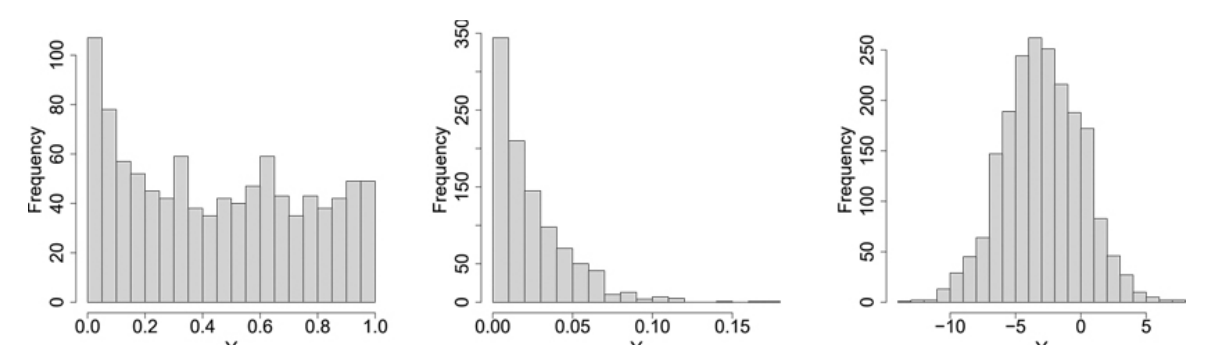
\includegraphics[width=0.95\linewidth]{ex04_histograms_book.png}
\item The data in this table

\smallskip
\centering
\begin{tabular}{cc}\toprule Failure & Success\\\midrule 799 & 202\\\bottomrule\end{tabular}
\end{enumerate}
\end{problem}

\begin{restate}
For each quantity, decide what kind of values it can take, then match it to a standard distribution.
\end{restate}

\begin{recall}
\begin{center}
\begin{tabular}{ll}\toprule
Possible values (support) & Natural families\\\midrule
$\{0,1\}$ (yes/no) & Bernoulli\\
$\{0,1,\dots,n\}$ (count out of a fixed $n$) & Binomial\\
$\{0,1,2,\dots\}$ (count with no upper limit) & Poisson, negative binomial\\
$(0,\infty)$ (positive, often skewed) & Exponential, Gamma, Log-normal, Weibull\\
$(0,1)$ (a proportion) & Beta\\
$(-\infty,\infty)$ (symmetric, bell-shaped) & Normal, Student-$t$\\\bottomrule
\end{tabular}
\end{center}
\end{recall}

\begin{keyidea}
Two questions, in this order: \textbf{(1) What values are possible?} \textbf{(2) What shape?} (symmetric or skewed; where is the peak?)
\end{keyidea}

\solution
\step{(a) Waiting time at Starbucks.}
\emph{Values:} positive, continuous. \emph{Shape:} right-skewed --- most orders take a few minutes, a few take much longer --- with the peak \emph{away} from zero.
$\Rightarrow$ \textbf{Gamma} with shape $>1$ (log-normal or Weibull also fine). The exponential is a poor choice because its peak is at 0.

\step{(b) Heart rate.}
\emph{Values:} continuous, around 60--100 bpm, far from 0. \emph{Shape:} roughly symmetric, bell-shaped.
$\Rightarrow$ \textbf{Normal} (with mean $\approx75$ and SD $\approx10$ it puts essentially no probability below 0).

\step{(c) Hurricanes per year.}
\emph{Values:} $0,1,2,\dots$, no fixed maximum; rare, roughly independent events.
$\Rightarrow$ \textbf{Poisson} (negative binomial if years vary more than a Poisson allows).

\step{(d) Adverse events among 100 patients.}
\emph{Values:} $0,1,\dots,100$ --- a count out of a fixed number of yes/no outcomes.
$\Rightarrow$ \textbf{Binomial}$(100,\theta)$.

\step{(e) The three histograms.}
\begin{itemize}
\item \emph{Left:} values only in $[0,1]$, a spike near 0, roughly flat elsewhere.
$\Rightarrow$ \textbf{Beta}$(a,b)$ with $a<1$ (the spike at 0) and $b$ near 1.
\item \emph{Middle:} positive values (0 to $\approx0.15$), highest bar at 0, long right tail.
$\Rightarrow$ \textbf{Exponential} (or Gamma with shape $\le1$).
\item \emph{Right:} symmetric bell centred near $-2.5$, negative and positive values.
$\Rightarrow$ \textbf{Normal} (roughly $\mu\approx-2.5$, $\sigma\approx2.5$).
\end{itemize}

\step{(f) Failure/success table.}
$799+202=1{,}001$ yes/no outcomes: each is \textbf{Bernoulli}$(\theta)$; the number of successes is \textbf{Binomial}$(1001,\theta)$.

\begin{answer}
(a) Gamma / log-normal \quad (b) Normal \quad (c) Poisson \quad (d) Binomial$(100,\theta)$\\
(e) Beta (left), Exponential (middle), Normal (right) \quad (f) Bernoulli trials $\Rightarrow$ Binomial$(1001,\theta)$
\end{answer}

\begin{takeaway}
There is rarely a single ``right'' family; the \emph{justification} (support, then shape) is what matters.
\end{takeaway}

% ================================================================= Exercise 5
\exercise{1.5 --- Building a prior from a mean and variance}

\begin{problem}{5}
Expert knowledge dictates that a parameter must be positive and that its prior distribution should have the mean 5 and variance 3. Find a prior distribution that satisfies these constraints.
\end{problem}

\begin{restate}
Pick a distribution that only takes positive values, then tune its two parameters so that its mean is 5 and its variance is 3.
\end{restate}

\begin{recall}
If $\theta\sim\dist{Gamma}(a,b)$ (shape $a$, rate $b$): density $\propto\theta^{a-1}e^{-b\theta}$ on $(0,\infty)$, \ $\E\theta=\frac ab$, \ $\V\theta=\frac a{b^2}$.
\end{recall}

\begin{keyidea}
\textbf{Moment matching}: two conditions (mean, variance), two unknowns $(a,b)$ $\Rightarrow$ solve two equations.
\end{keyidea}

\solution
\step{Step 1 --- choose a family.}
The parameter is positive, so we need a distribution on $(0,\infty)$; the Gamma is the standard choice.

\step{Step 2 --- write the two equations.}
\[
\text{(i)}\ \ \frac ab=5,\qquad\text{(ii)}\ \ \frac{a}{b^2}=3.
\]

\step{Step 3 --- solve.}
Divide (i) by (ii): $\dfrac{a/b}{a/b^2}=\dfrac{a}{b}\cdot\dfrac{b^2}{a}=b$, so $b=\dfrac53\approx1.667$.
Then from (i): $a=5b=\dfrac{25}{3}\approx8.333$.

\step{Step 4 --- an alternative family (log-normal).}
If $\log\theta\sim\dist{Normal}(\mu,\sigma^2)$, then $\E\theta=e^{\mu+\sigma^2/2}$ and $\V\theta=(e^{\sigma^2}-1)(\E\theta)^2$. So $e^{\sigma^2}-1=\frac{3}{25}$, giving $\sigma^2=\log(1.12)=0.1133$ and $\mu=\log5-\frac{\sigma^2}2=1.5528$.

\begin{sanity}
Mean $\frac{25/3}{5/3}=5$ \checkmark; \ variance $\frac{25/3}{(5/3)^2}=\frac{25/3}{25/9}=3$ \checkmark.
\end{sanity}

\begin{answer}
$\theta\sim\dist{Gamma}\big(a=\tfrac{25}{3},\ b=\tfrac53\big)$ (shape--rate): positive, mean 5, variance 3.
(Equally valid: $\theta\sim\dist{LogNormal}(1.5528,\,0.1133)$.)
\end{answer}

\begin{takeaway}
\begin{itemize}
\item A $\dist{Normal}(5,3)$ prior would be \textbf{wrong}: it gives $\Prob(\theta<0)=\Phi(-5/\sqrt3)\approx0.002>0$.
\item Watch the parameterisation: in the shape--\emph{scale} form the scale is $1/b=0.6$.
\end{itemize}
\end{takeaway}

% ================================================================= Exercise 6
\exercise{1.6 --- Marginal and conditional distributions from a table}

\begin{problem}{6}
$X_1$ and $X_2$ have joint PMF
\begin{center}
\begin{tabular}{cc|c}\toprule
$x_1$ & $x_2$ & $\Prob(X_1=x_1, X_2=x_2)$\\\midrule
0&0&0.15\\ 1&0&0.15\\ 2&0&0.15\\ 0&1&0.15\\ 1&1&0.20\\ 2&1&0.20\\\bottomrule
\end{tabular}
\end{center}
\begin{enumerate}[(a)]
\item Compute the marginal distribution of $X_1$.
\item Compute the marginal distribution of $X_2$.
\item Compute the conditional distribution of $X_1|X_2$.
\item Compute the conditional distribution of $X_2|X_1$.
\item Are $X_1$ and $X_2$ independent? Justify your answer.
\end{enumerate}
\end{problem}

\begin{restate}
From a table of joint probabilities, find each variable's own distribution, the distribution of one given the other, and check whether they influence each other.
\end{restate}

\begin{recall}
\begin{itemize}
\item \textbf{Marginal}: add up the joint probabilities over the other variable.
\item \textbf{Conditional}: joint $\div$ marginal of the variable you condition on.
\item \textbf{Independence}: joint $=$ product of marginals in \emph{every} cell.
\end{itemize}
\end{recall}

\begin{keyidea}
Rearrange the list into a $2\times3$ grid: marginals are row and column totals, and conditionals are rows (or columns) rescaled to add to 1.
\end{keyidea}

\solution
\step{Step 0 --- the grid with totals.}
\begin{center}
\begin{tabular}{c|ccc|c}\toprule
 & $x_1=0$ & $x_1=1$ & $x_1=2$ & row total $=\Prob(X_2=x_2)$\\\midrule
$x_2=0$ & 0.15 & 0.15 & 0.15 & \textbf{0.45}\\
$x_2=1$ & 0.15 & 0.20 & 0.20 & \textbf{0.55}\\\midrule
column total $=\Prob(X_1=x_1)$ & \textbf{0.30} & \textbf{0.35} & \textbf{0.35} & 1.00\\\bottomrule
\end{tabular}
\end{center}

\step{(a) Marginal of $X_1$} (add each column):
$\Prob(X_1=0)=0.15+0.15=0.30$, \ $\Prob(X_1=1)=0.15+0.20=0.35$, \ $\Prob(X_1=2)=0.15+0.20=0.35$.

\step{(b) Marginal of $X_2$} (add each row):
$\Prob(X_2=0)=0.15+0.15+0.15=0.45$, \ $\Prob(X_2=1)=0.15+0.20+0.20=0.55$.

\step{(c) Conditional of $X_1$ given $X_2$} (divide each row by its total):
\begin{center}
\begin{tabular}{c|ccc|c}\toprule
 & $x_1=0$ & $x_1=1$ & $x_1=2$ & sum\\\midrule
$X_2=0$ & $\frac{0.15}{0.45}=\frac13$ & $\frac{0.15}{0.45}=\frac13$ & $\frac{0.15}{0.45}=\frac13$ & 1\\[3pt]
$X_2=1$ & $\frac{0.15}{0.55}=\frac{3}{11}\approx0.273$ & $\frac{0.20}{0.55}=\frac{4}{11}\approx0.364$ & $\frac4{11}\approx0.364$ & 1\\\bottomrule
\end{tabular}
\end{center}
\why{$\Prob(X_1=x_1\mid X_2=x_2)=\Prob(X_1=x_1,X_2=x_2)/\Prob(X_2=x_2)$: we zoom into one row and rescale it to sum to 1.}

\step{(d) Conditional of $X_2$ given $X_1$} (divide each column by its total):
\begin{center}
\begin{tabular}{c|cc|c}\toprule
 & $x_2=0$ & $x_2=1$ & sum\\\midrule
$X_1=0$ & $\frac{0.15}{0.30}=\frac12$ & $\frac{0.15}{0.30}=\frac12$ & 1\\[3pt]
$X_1=1$ & $\frac{0.15}{0.35}=\frac37\approx0.429$ & $\frac{0.20}{0.35}=\frac47\approx0.571$ & 1\\[3pt]
$X_1=2$ & $\frac37\approx0.429$ & $\frac47\approx0.571$ & 1\\\bottomrule
\end{tabular}
\end{center}

\step{(e) Independence?}
Test one cell: $\Prob(X_1=0,X_2=0)=0.15$, but $\Prob(X_1=0)\cdot\Prob(X_2=0)=0.30\times0.45=0.135$. Since $0.15\neq0.135$, they are \textbf{not independent}. Equivalently, the conditional of $X_1$ changes with $X_2$ ($\frac13$ vs.\ $\frac3{11}$ for $x_1=0$).

\begin{sanity}
Every conditional row/column sums to 1, and each marginal sums to 1. \checkmark
\end{sanity}

\begin{answer}
(a) $X_1$: $(0.30, 0.35, 0.35)$ on $(0,1,2)$. \quad (b) $X_2$: $(0.45, 0.55)$ on $(0,1)$.\\
(c) $X_1|X_2=0$: $(\frac13,\frac13,\frac13)$;\quad $X_1|X_2=1$: $(\frac3{11},\frac4{11},\frac4{11})$.\\
(d) $X_2|X_1=0$: $(\frac12,\frac12)$;\quad $X_2|X_1=1$ and $X_2|X_1=2$: $(\frac37,\frac47)$.\\
(e) \textbf{Not independent}: $0.15\neq0.30\times0.45=0.135$.
\end{answer}

\begin{takeaway}
Proving independence requires checking \emph{every} cell; disproving it needs just one counter-example.
\end{takeaway}

% ================================================================= Exercise 7
\exercise{1.7 --- The bivariate normal: marginal and conditional}

\begin{problem}{7}
If $(X_1,X_2)$ is bivariate normal with $\E(X_1)=\E(X_2)=0$, $\V(X_1)=\V(X_2)=1$, and $\Cor(X_1,X_2)=\rho$:
\begin{enumerate}[(a)]
\item Derive the marginal distribution of $X_1$.
\item Derive the conditional distribution of $X_1|X_2$.
\end{enumerate}
\end{problem}

\begin{restate}
Starting from the joint bell-shaped density of two correlated standard normals, show that $X_1$ on its own is standard normal, and find the distribution of $X_1$ once $X_2$ is known.
\end{restate}

\begin{recall}
\begin{itemize}
\item Joint density (unit variances, correlation $\rho$, $|\rho|<1$):
$f(x_1,x_2)=\dfrac{1}{2\pi\sqrt{1-\rho^2}}\exp\Big\{-\dfrac{x_1^2-2\rho x_1x_2+x_2^2}{2(1-\rho^2)}\Big\}$.
\item \textbf{Gaussian integral}: $\displaystyle\int_{-\infty}^\infty\exp\Big\{-\frac{(z-m)^2}{2v}\Big\}\dd z=\sqrt{2\pi v}$ for any $m$ and $v>0$.
\item \textbf{Completing the square}: $z^2-2bz=(z-b)^2-b^2$.
\end{itemize}
\end{recall}

\begin{keyidea}
Complete the square so one variable appears only inside a single squared term; then it integrates out with the Gaussian integral.
\end{keyidea}

\solution
\step{Step 1 --- complete the square in $x_2$.}
Using $z^2-2bz=(z-b)^2-b^2$ with $z=x_2$ and $b=\rho x_1$:
\[
x_2^2-2\rho x_1x_2=(x_2-\rho x_1)^2-\rho^2x_1^2,
\]
so
\[
x_1^2-2\rho x_1x_2+x_2^2=(x_2-\rho x_1)^2+x_1^2-\rho^2x_1^2=(x_2-\rho x_1)^2+(1-\rho^2)x_1^2.
\]

\step{Step 2 --- split the exponent.}
Divide by $2(1-\rho^2)$:
\[
\frac{(x_2-\rho x_1)^2+(1-\rho^2)x_1^2}{2(1-\rho^2)}=\frac{(x_2-\rho x_1)^2}{2(1-\rho^2)}+\frac{x_1^2}{2}.
\]
So the joint density factors as
\[
f(x_1,x_2)=\frac{1}{2\pi\sqrt{1-\rho^2}}\ e^{-x_1^2/2}\ \exp\Big\{-\frac{(x_2-\rho x_1)^2}{2(1-\rho^2)}\Big\}.
\]

\step{(a) Step 3 --- integrate out $x_2$.}
The last factor is a Gaussian integral in $x_2$ with $m=\rho x_1$ and $v=1-\rho^2$; it equals $\sqrt{2\pi(1-\rho^2)}$:
\[
f(x_1)=\int f(x_1,x_2)\dd x_2=\frac{\sqrt{2\pi(1-\rho^2)}}{2\pi\sqrt{1-\rho^2}}\,e^{-x_1^2/2}=\frac{1}{\sqrt{2\pi}}\,e^{-x_1^2/2}.
\]
\why{$\frac{\sqrt{2\pi}\sqrt{1-\rho^2}}{2\pi\sqrt{1-\rho^2}}=\frac{\sqrt{2\pi}}{2\pi}=\frac{1}{\sqrt{2\pi}}$.}
This is exactly the $\dist{Normal}(0,1)$ density.

\step{(b) Step 4 --- conditional = joint / marginal.}
By symmetry $f(x_2)=\frac1{\sqrt{2\pi}}e^{-x_2^2/2}$, and completing the square in $x_1$ instead gives
\[
f(x_1,x_2)=\frac{1}{2\pi\sqrt{1-\rho^2}}\,e^{-x_2^2/2}\exp\Big\{-\frac{(x_1-\rho x_2)^2}{2(1-\rho^2)}\Big\}.
\]
Dividing,
\[
f(x_1\mid x_2)=\frac{f(x_1,x_2)}{f(x_2)}=\frac{\sqrt{2\pi}}{2\pi\sqrt{1-\rho^2}}\exp\Big\{-\frac{(x_1-\rho x_2)^2}{2(1-\rho^2)}\Big\}
=\frac{1}{\sqrt{2\pi(1-\rho^2)}}\exp\Big\{-\frac{(x_1-\rho x_2)^2}{2(1-\rho^2)}\Big\},
\]
the $\dist{Normal}(\rho x_2,\ 1-\rho^2)$ density.

\begin{sanity}
If $\rho=0$: conditional $=\dist N(0,1)=$ marginal (independence). If $\rho\to1$: conditional variance $\to0$ and mean $\to x_2$, i.e.\ $X_1=X_2$. Both limits make sense.
\end{sanity}

\begin{answer}
(a) $X_1\sim\dist{Normal}(0,1)$. \qquad (b) $X_1\mid X_2=x_2\ \sim\ \dist{Normal}\big(\rho x_2,\ 1-\rho^2\big)$.
\end{answer}

\begin{takeaway}
\begin{itemize}
\item The conditional mean $\rho x_2$ is a straight line with slope $\rho$ --- the origin of linear regression.
\item The conditional variance $1-\rho^2\le1$: knowing $X_2$ always reduces uncertainty about $X_1$.
\end{itemize}
\end{takeaway}

% ================================================================= Exercise 8
\exercise{1.8 --- Uncorrelated but dependent}

\begin{problem}{8}
Assume $(X_1,X_2)$ have support $X_1,X_2\in\mathbb R$ and bivariate PDF
\[
f(x_1,x_2)=\frac{1}{2\pi}\big(1+x_1^2+x_2^2\big)^{-3/2}.
\]
\begin{enumerate}[(a)]
\item Plot the conditional distribution of $X_1|X_2=x_2$ for $x_2\in\{-3,-2,-1,0,1,2,3\}$ (preferably on the same plot).
\item Do $X_1$ and $X_2$ appear to be correlated? Justify your answer.
\item Do $X_1$ and $X_2$ appear to be independent? Justify your answer.
\end{enumerate}
\end{problem}

\begin{restate}
Look at how the distribution of $X_1$ changes as we fix $X_2$ at different values. Is there a linear trend (correlation)? Is there any dependence at all?
\end{restate}

\begin{recall}
\begin{itemize}
\item \textbf{Correlation} measures only a \emph{linear} relationship: does the \emph{centre} of $X_1$ move as $x_2$ changes?
\item \textbf{Independence} requires the \emph{entire} conditional distribution (centre, spread, shape) to be the same for every $x_2$.
\item Useful integral: $\displaystyle\int_{-\infty}^\infty(A+t^2)^{-3/2}\dd t=\frac{2}{A}$ for $A>0$ (substitute $t=\sqrt A\tan u$).
\end{itemize}
\end{recall}

\begin{keyidea}
Compute $f(x_1\mid x_2)$ in closed form and see which features depend on $x_2$.
\end{keyidea}

\solution
\step{Step 1 --- marginal of $X_2$.}
Fix $x_2$ and let $A=1+x_2^2$. Then
\[
f(x_2)=\frac1{2\pi}\int_{-\infty}^\infty(A+x_1^2)^{-3/2}\dd x_1=\frac{1}{2\pi}\cdot\frac{2}{A}=\frac{1}{\pi(1+x_2^2)},
\]
the \textbf{standard Cauchy} density. By symmetry, $X_1$ is standard Cauchy too.

\step{Step 2 --- the conditional density.}
\[
f(x_1\mid x_2)=\frac{f(x_1,x_2)}{f(x_2)}=\frac{\frac1{2\pi}(A+x_1^2)^{-3/2}}{\frac{1}{\pi A}}=\frac{A}{2}\,(A+x_1^2)^{-3/2}.
\]
Write $a=\sqrt A=\sqrt{1+x_2^2}$ and pull $a^2$ out of the bracket:
\[
f(x_1\mid x_2)=\frac{a^2}{2}\,a^{-3}\Big(1+\frac{x_1^2}{a^2}\Big)^{-3/2}=\frac{1}{2a}\Big(1+\frac{x_1^2}{a^2}\Big)^{-3/2}.
\]
This is a Student-$t$ density with 2 degrees of freedom, centred at 0, with scale $a/\sqrt2$. Its peak height is $\frac{1}{2a}$.

\step{(a) The plot.}
\begin{center}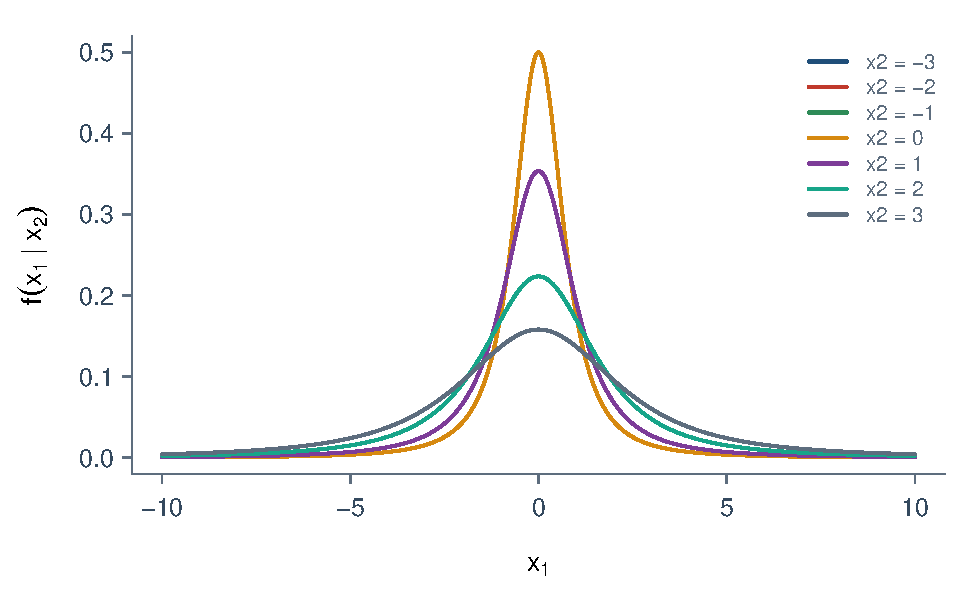
\includegraphics[width=0.78\linewidth]{ex08_conditionals.pdf}\end{center}
All curves are centred at 0. As $|x_2|$ grows the curve gets lower and wider (peak 0.50 at $x_2=0$, 0.158 at $|x_2|=3$); curves for $\pm x_2$ coincide.

\step{(b) Correlated?}
\textbf{No linear trend.} The centre of $X_1\mid X_2=x_2$ is 0 for every $x_2$, and $f(x_1,x_2)=f(-x_1,x_2)$, so large $X_2$ is no more likely to come with large $X_1$ than with small $X_1$. (Strictly, the correlation is not even defined, because Cauchy variables have infinite variance.)

\step{(c) Independent?}
\textbf{No.} If they were independent all seven curves would be identical; instead the \emph{spread} of $X_1$ grows with $|x_2|$. One cell proves it: $f(0,0)=\frac1{2\pi}=0.159$, but $f_1(0)f_2(0)=\frac1\pi\cdot\frac1\pi=0.101$.

\begin{sanity}
Each conditional curve integrates to 1 (checked numerically in \texttt{ch01.R}: all seven integrals equal 1.0000).
\end{sanity}

\begin{answer}
(a) All conditionals are symmetric about 0 and get wider as $|x_2|$ grows ($X_1\mid x_2$ is a $t_2$ with scale $\sqrt{(1+x_2^2)/2}$).
(b) \textbf{Not} correlated --- the centre never moves. (c) \textbf{Not} independent --- the spread changes with $x_2$.
\end{answer}

\begin{takeaway}
\textbf{Uncorrelated does not imply independent.} Correlation cannot see dependence that lives in the spread. (For the bivariate normal of Exercise 7 the two notions coincide.)
\end{takeaway}

% ================================================================= Exercise 9
\exercise{1.9 --- Car thefts in the Triangle}

\begin{problem}{9}
According to insurance.com, the 2017 auto theft rate was 135 per 10,000 residents in Raleigh, NC compared to 214 per 10,000 residents in Durham/Chapel Hill, NC. Assuming Raleigh's population is twice as large as Durham/Chapel Hill and a car has been stolen somewhere in the triangle (i.e., one of these two areas), what the probability it was stolen in Raleigh?
\end{problem}

\begin{restate}
Raleigh has a lower theft \emph{rate} but twice the people. Given that a theft happened, which city is it more likely to have been in?
\end{restate}

\begin{recall}
Bayes' rule with two hypotheses ($R$ = Raleigh, $D$ = Durham/Chapel Hill) and data $T$ (a theft occurred):
$\Prob(R\mid T)=\dfrac{\Prob(T\mid R)\Prob(R)}{\Prob(T\mid R)\Prob(R)+\Prob(T\mid D)\Prob(D)}$.
\end{recall}

\begin{keyidea}
\textbf{Prior} = share of the population; \textbf{likelihood} = theft rate in that city.
\end{keyidea}

\solution
\step{Step 1 --- prior.} Out of every 3 residents, 2 live in Raleigh: $\Prob(R)=\frac23$, $\Prob(D)=\frac13$.

\step{Step 2 --- likelihoods.} $\Prob(T\mid R)=\frac{135}{10{,}000}=0.0135$ and $\Prob(T\mid D)=\frac{214}{10{,}000}=0.0214$.

\step{Step 3 --- numerator and denominator.}
\[
\Prob(T\mid R)\Prob(R)=0.0135\times\tfrac23=0.009000,\qquad\Prob(T\mid D)\Prob(D)=0.0214\times\tfrac13=0.007133.
\]
\step{Step 4 --- posterior.}
\[
\Prob(R\mid T)=\frac{0.009000}{0.009000+0.007133}=\frac{0.009000}{0.016133}=0.558.
\]

\begin{sanity}
\textbf{Counting version.} Imagine 10{,}000 people in Durham/Chapel Hill and 20{,}000 in Raleigh. Expected thefts: $214$ and $2\times135=270$. Out of $484$ thefts, $270$ are in Raleigh: $270/484=0.558$. \checkmark
\end{sanity}

\begin{answer}
$\Prob(\text{Raleigh}\mid\text{car stolen})=270/484\approx\mathbf{0.558}$.
\end{answer}

\begin{takeaway}
Ignoring the prior and answering $135/(135+214)=0.387$ is the classic \emph{base-rate fallacy}.
\end{takeaway}

% ================================================================= Exercise 10
\exercise{1.10 --- Spam filter}

\begin{problem}{10}
Say 60\% of the emails that arrive in your inbox are spam. Your account correctly flags spam emails as spam with probability 95\% and incorrectly flags other emails as spam with probability 2\%. Given that an email is flagged as spam, what is the probability it is actually a spam email?
\end{problem}

\begin{restate}
If the filter says ``spam'', how likely is it really spam?
\end{restate}

\begin{recall}
Law of total probability: $\Prob(F)=\Prob(F\mid S)\Prob(S)+\Prob(F\mid S^c)\Prob(S^c)$. Bayes' rule: $\Prob(S\mid F)=\Prob(F\mid S)\Prob(S)/\Prob(F)$.
\end{recall}

\begin{keyidea}
Prior $\Prob(S)=0.6$; likelihoods $\Prob(F\mid S)=0.95$ (sensitivity) and $\Prob(F\mid S^c)=0.02$ (false-alarm rate).
\end{keyidea}

\solution
\step{Step 1 --- probability an email is flagged.}
$\Prob(F)=0.95\times0.6+0.02\times0.4=0.570+0.008=0.578$.
\step{Step 2 --- Bayes' rule.}
$\Prob(S\mid F)=\dfrac{0.95\times0.6}{0.578}=\dfrac{0.570}{0.578}=0.9862$.

\begin{sanity}
\textbf{Counting version.} Of 1{,}000 emails, 600 are spam and 570 of them are flagged; 400 are genuine and 8 of them are flagged. Of the 578 flagged, 570 are spam: $570/578=0.986$. \checkmark
\end{sanity}

\begin{answer}
$\Prob(\text{spam}\mid\text{flagged})=0.570/0.578\approx\mathbf{0.986}$.
\end{answer}

\begin{takeaway}
The high base rate (60\%) is why a flag is so reliable here. If only 1\% of emails were spam, the same filter would give $\frac{0.0095}{0.0095+0.0198}=0.32$.
\end{takeaway}

% ================================================================= Exercise 11
\exercise{1.11 --- Commute times and conventions}

\begin{problem}{11}
Your daily commute is distributed uniformly between 15 and 20 minutes if there is no convention downtown. However, conventions are scheduled for roughly 1 in 4 days, and your commute time is distributed uniformly from 15 to 30 minutes if there is a convention. Let $Y$ be your commute time this morning.
\begin{enumerate}[(a)]
\item What is the probability that there was a convention downtown given $Y=18$?
\item What is the probability that there was a convention downtown given $Y=28$?
\end{enumerate}
\end{problem}

\begin{restate}
From today's commute time, work out how likely it is that there was a convention.
\end{restate}

\begin{recall}
For a \textbf{continuous} observation, Bayes' rule uses \emph{densities} in place of probabilities of the data:
$\Prob(C\mid Y=y)=\dfrac{f(y\mid C)\Prob(C)}{f(y\mid C)\Prob(C)+f(y\mid C^c)\Prob(C^c)}$.
A $\dist{Uniform}(a,b)$ density is $\frac1{b-a}$ inside $[a,b]$ and 0 outside.
\end{recall}

\begin{keyidea}
Prior $\Prob(C)=\frac14$. Likelihoods: $f(y\mid C)=\frac1{15}$ on $[15,30]$; $f(y\mid C^c)=\frac15$ on $[15,20]$, 0 elsewhere.
\end{keyidea}

\solution
\step{(a) $Y=18$.} Both scenarios can produce 18 minutes:
\[
\Prob(C\mid Y=18)=\frac{\frac14\cdot\frac1{15}}{\frac14\cdot\frac1{15}+\frac34\cdot\frac15}=\frac{\frac1{60}}{\frac1{60}+\frac{9}{60}}=\frac{1}{10}=0.10.
\]
\why{$\frac34\cdot\frac15=\frac3{20}=\frac9{60}$; then the $\frac1{60}$'s cancel.}
\step{(b) $Y=28$.} Without a convention a 28-minute commute is impossible, $f(28\mid C^c)=0$:
\[
\Prob(C\mid Y=28)=\frac{\frac14\cdot\frac1{15}}{\frac14\cdot\frac1{15}+\frac34\cdot0}=1.
\]

\begin{sanity}
In (a) the posterior (0.10) is \emph{below} the prior (0.25): 18 minutes is 3 times more likely on a normal day (density $\frac15$) than on a convention day ($\frac1{15}$). \checkmark
\end{sanity}

\begin{answer}
(a) $\Prob(C\mid Y=18)=\mathbf{0.10}$ \qquad (b) $\Prob(C\mid Y=28)=\mathbf{1}$
\end{answer}

\begin{takeaway}
Any $Y\in[15,20]$ gives the same answer 0.1 (both likelihoods are flat there); any $Y\in(20,30]$ proves there was a convention.
\end{takeaway}

% ================================================================= Exercise 12
\exercise{1.12 --- Aleatoric vs.\ epistemic uncertainty}

\begin{problem}{12}
Consider the problem of short-term weather forecasting. Describe (i) a potential source of aleatoric uncertainty and (ii) a potential source of epistemic uncertainty.
\end{problem}

\begin{restate}
Give one source of randomness that no extra knowledge could remove, and one source of uncertainty that comes from what we do not (yet) know.
\end{restate}

\begin{recall}
\textbf{Aleatoric} (Latin \emph{alea}, ``dice''): inherent randomness in the outcome, even if the model and its parameters were known exactly --- lives in the likelihood $f(Y\mid\theta)$.
\textbf{Epistemic} (Greek \emph{episteme}, ``knowledge''): uncertainty due to limited knowledge of parameters or model --- lives in the posterior $p(\theta\mid Y)$ and shrinks with more data.
\end{recall}

\begin{keyidea}
Test: \emph{would more data or a better model make this uncertainty disappear?} Yes $\Rightarrow$ epistemic; no $\Rightarrow$ aleatoric.
\end{keyidea}

\solution
\step{(i) Aleatoric.}
The atmosphere is chaotic: tiny, unmeasurable turbulent fluctuations decide whether a shower forms over \emph{this} neighbourhood in the next hour. Even with a perfect model and perfect parameters, ``will it rain at my house at 3 pm'' remains genuinely random --- hence forecasts like ``40\% chance of rain''.

\step{(ii) Epistemic.}
Imperfect knowledge of the inputs and the model: the current state of the atmosphere over areas with few weather stations (e.g.\ oceans), or uncertain parameters in how the forecast model represents clouds. More observations and better calibration reduce this.

\begin{answer}
(i) Aleatoric: chaotic small-scale variability (exactly where a storm cell forms). (ii) Epistemic: imperfectly known initial conditions / model parameters due to limited observations --- reducible with more data.
\end{answer}

\begin{takeaway}
The posterior predictive distribution (Section 1.5) combines both: it averages the aleatoric spread $f(Y^*\mid\theta)$ over the epistemic uncertainty $p(\theta\mid Y)$.
\end{takeaway}

% ================================================================= Exercise 13
\exercise{1.13 --- A Bayesian spell checker}

\begin{problem}{13}
For this problem pretend we are dealing with a language with a six-word dictionary
\[
\{\text{fun, sun, sit, sat, fan, for}\}.
\]
An extensive study of literature written in this language reveals that all words are equally likely except that ``for'' is $\alpha$ times as likely as the other words. Further study reveals that:
\begin{enumerate}[i.]
\item Each keystroke is an error with probability $\theta$.
\item All letters are equally likely to produce errors.
\item Given that a letter is typed incorrectly it is equally likely to be any other letter.
\item Errors are independent across letters.
\end{enumerate}
For example, the probability of correctly typing ``fun'' (or any other word) is $(1-\theta)^3$, the probability of typing ``pun'' or ``fon'' when intending to type is ``fun'' is $\theta(1-\theta)^2$, and the probability of typing ``foo'' or ``nnn'' when intending to type ``fun'' is $\theta^2(1-\theta)$. Use Bayes' rule to develop a simple spell checker for this language. For each of the typed words ``sun'', ``the'', ``foo'', give the probability that each word in the dictionary was the intended word. Perform this for the parameters below:
\begin{enumerate}[(a)]
\item $\alpha=2$ and $\theta=0.1$.
\item $\alpha=50$ and $\theta=0.1$.
\item $\alpha=2$ and $\theta=0.95$.
\end{enumerate}
Comment on the changes you observe in these three cases.
\end{problem}

\begin{restate}
Someone typed a 3-letter string. Combine (1) how common each dictionary word is and (2) how likely that typo is, to get the probability of each intended word.
\end{restate}

\begin{recall}
Bayes' rule over six hypotheses $w\in\{\text{fun},\dots,\text{for}\}$:
$\Prob(w\mid t)=\dfrac{\Prob(t\mid w)\Prob(w)}{\sum_{w'}\Prob(t\mid w')\Prob(w')}$.
\end{recall}

\begin{keyidea}
\textbf{Prior}: $\Prob(\text{for})=\frac{\alpha}{5+\alpha}$, every other word $\frac1{5+\alpha}$. \textbf{Likelihood}: if $w$ and $t$ differ in $k$ positions, $\Prob(t\mid w)=\theta^k(1-\theta)^{3-k}$ (as in the exercise's examples).
\end{keyidea}

\solution
\step{Step 1 --- the prior.}
The weights are $1,1,1,1,1,\alpha$ for (fun, sun, sit, sat, fan, for); they sum to $5+\alpha$.

\step{Step 2 --- count mismatches $k(w,t)$} (compare letter by letter):
\begin{center}
\begin{tabular}{l|cccccc}\toprule
typed $t$ & fun & sun & sit & sat & fan & for\\\midrule
sun & 1 & 0 & 2 & 2 & 2 & 3\\
the & 3 & 3 & 3 & 3 & 3 & 3\\
foo & 2 & 3 & 3 & 3 & 2 & 1\\\bottomrule
\end{tabular}
\end{center}
\why{Example: ``sun'' vs.\ ``sit'': s=s, u$\neq$i, n$\neq$t $\Rightarrow k=2$.}

\step{Step 3 --- a simplification.}
$\theta^k(1-\theta)^{3-k}=(1-\theta)^3\,r^k$ with $r=\frac{\theta}{1-\theta}$. The common factor $(1-\theta)^3$ cancels, so
\[
\Prob(w\mid t)=\frac{\pi_w\,r^{k(w,t)}}{\sum_{w'}\pi_{w'}\,r^{k(w',t)}}.
\]
For $\theta=0.1$: $r=\frac19$ --- each extra typo makes a word 9 times less likely. For $\theta=0.95$: $r=19$ --- each extra typo makes a word 19 times \emph{more} likely.

\step{Step 4 --- worked example: case (a), typed ``sun''.}
Unnormalised weights $\pi_w r^k$ (prior weights $1,\dots,1,2$):
\begin{center}
\begin{tabular}{lcccccc}\toprule
 & fun & sun & sit & sat & fan & for\\\midrule
weight & $1\cdot\frac19$ & $1\cdot1$ & $1\cdot\frac1{81}$ & $\frac1{81}$ & $\frac1{81}$ & $2\cdot\frac1{729}$\\
value & 0.1111 & 1.0000 & 0.0123 & 0.0123 & 0.0123 & 0.0027\\\bottomrule
\end{tabular}
\end{center}
Total $=1.1509$, so $\Prob(\text{sun}\mid\text{sun})=\frac{1}{1.1509}=0.869$, $\Prob(\text{fun}\mid\text{sun})=\frac{0.1111}{1.1509}=0.097$, etc.

\step{Step 5 --- all results} (from \texttt{ch01.R}):
\begin{center}
\small
\begin{tabular}{cl|cccccc}\toprule
case & typed & fun & sun & sit & sat & fan & for\\\midrule
\multirow{3}{*}{(a) $\alpha=2,\theta=0.1$}
 & sun & 0.097 & \textbf{0.869} & 0.011 & 0.011 & 0.011 & 0.002\\
 & the & 0.143 & 0.143 & 0.143 & 0.143 & 0.143 & \textbf{0.286}\\
 & foo & 0.049 & 0.006 & 0.006 & 0.006 & 0.049 & \textbf{0.885}\\\midrule
\multirow{3}{*}{(b) $\alpha=50,\theta=0.1$}
 & sun & 0.091 & \textbf{0.822} & 0.010 & 0.010 & 0.010 & 0.056\\
 & the & 0.018 & 0.018 & 0.018 & 0.018 & 0.018 & \textbf{0.909}\\
 & foo & 0.002 & 0.000 & 0.000 & 0.000 & 0.002 & \textbf{0.995}\\\midrule
\multirow{3}{*}{(c) $\alpha=2,\theta=0.95$}
 & sun & 0.001 & 0.000 & 0.024 & 0.024 & 0.024 & \textbf{0.926}\\
 & the & 0.143 & 0.143 & 0.143 & 0.143 & 0.143 & \textbf{0.286}\\
 & foo & 0.017 & \textbf{0.322} & \textbf{0.322} & \textbf{0.322} & 0.017 & 0.002\\\bottomrule
\end{tabular}
\end{center}

\step{Step 6 --- comments.}
\begin{itemize}
\item \textbf{``the''} differs from every word in all 3 letters, so all likelihoods are equal and the \textbf{posterior equals the prior} ($\frac27=0.286$ for ``for'' when $\alpha=2$; $\frac{50}{55}=0.909$ when $\alpha=50$).
\item \textbf{(a) $\to$ (b):} a larger $\alpha$ moves probability toward ``for''. Clear evidence (``sun'' typed, a perfect match) still wins (0.82), but weak evidence gives way to the prior.
\item \textbf{(c) $\theta=0.95$:} the typist almost always hits the wrong key, so a \emph{matching} letter is evidence \emph{against} a word. The checker now prefers the words that differ most.
\end{itemize}

\begin{note}
Rule iii strictly implies that a \emph{specific} wrong letter has probability $\theta/25$, i.e.\ likelihood $(\theta/25)^k(1-\theta)^{3-k}$. The book's worked example uses $\theta^k(1-\theta)^{3-k}$, so the table follows the book. Under the strict rule case (c) is much milder (e.g.\ ``sun'' $\to$ sun 0.229, for 0.201, fun 0.174). \texttt{ch01.R} prints both versions.
\end{note}

\begin{sanity}
Each row of the table sums to 1 (up to rounding). \checkmark
\end{sanity}

\begin{answer}
See the table. Posterior $\propto$ prior $\times\,\theta^k(1-\theta)^{3-k}$. ``the'' always returns the prior; larger $\alpha$ pulls ambiguous inputs toward ``for''; with $\theta=0.95$ the checker favours words that \emph{disagree} most with what was typed.
\end{answer}

\begin{takeaway}
This is how real noisy-channel spell checkers work: \emph{language model} (prior) $\times$ \emph{error model} (likelihood).
\end{takeaway}

% ================================================================= Exercise 14
\exercise{1.14 --- The zero-inflated Poisson}

\begin{problem}{14}
If $Y$ follows the Zero-Inflated Poisson (ZIP) distribution, it can be written in terms of two variables $Y=UV$, where $U\sim\dist{Bernoulli}(p)$ independent of $V\sim\dist{Poisson}(\lambda)$.
\begin{enumerate}[(a)]
\item Generate and plot a sample of size $n=10{,}000$ with $p=0.2$ and $\lambda=4$.
\item What is a real-life example of a variable that might follow this distribution? In your example, what are the interpretations of $U$ and $V$?
\item What is the probability that $Y=0$?
\item What is the probability that $Y=4$?
\item What is the probability that $U=0$ given that $Y=0$?
\item What is the probability that $U=0$ given that $Y=4$?
\end{enumerate}
\end{problem}

\begin{restate}
$Y$ is a count that is forced to 0 whenever a coin $U$ shows 0; otherwise it is a Poisson count. Simulate it, interpret it and compute some (conditional) probabilities.
\end{restate}

\begin{recall}
\begin{itemize}
\item $\Prob(V=v)=e^{-\lambda}\lambda^v/v!$; \quad $\Prob(V=0)=e^{-\lambda}$.
\item Law of total probability over $U$: $\Prob(Y=y)=\Prob(Y=y\mid U=0)\Prob(U=0)+\Prob(Y=y\mid U=1)\Prob(U=1)$.
\end{itemize}
\end{recall}

\begin{keyidea}
There are \textbf{two routes to $Y=0$}: a ``structural'' zero ($U=0$) or a ``Poisson'' zero ($U=1$ and $V=0$). Any positive value can only come from $U=1$.
\end{keyidea}

\solution
\step{(a) Simulation.}
\begin{lstlisting}
U <- rbinom(10000, 1, 0.2); V <- rpois(10000, 4); Y <- U * V
\end{lstlisting}
\begin{center}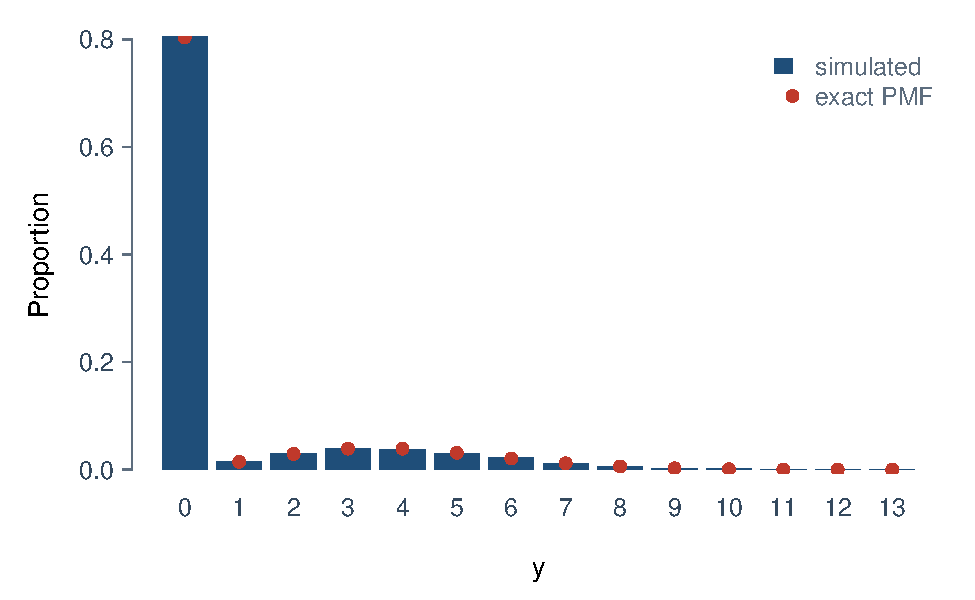
\includegraphics[width=0.75\linewidth]{ex14_zip.pdf}\end{center}
About 80\% of draws are zero; the rest look like a Poisson(4) scaled down by 0.2. Red dots: exact PMF.

\step{(b) Example.}
$Y$ = number of fish caught by a visitor to a park. $U$ = did the visitor go fishing at all; $V$ = number of fish caught if they did. (Also: cigarettes per day, with $U$ = is a smoker.)

\step{(c) $\Prob(Y=0)$.}
\[
\Prob(Y=0)=\underbrace{\Prob(U=0)}_{0.8}\cdot1+\underbrace{\Prob(U=1)}_{0.2}\cdot\underbrace{\Prob(V=0)}_{e^{-4}=0.01832}=0.8+0.00366=\mathbf{0.8037}.
\]
\step{(d) $\Prob(Y=4)$.} Only possible if $U=1$ and $V=4$:
\[
\Prob(Y=4)=0.2\cdot\frac{e^{-4}4^4}{4!}=0.2\cdot\frac{0.01832\times256}{24}=0.2\times0.1954=\mathbf{0.0391}.
\]
\step{(e) $\Prob(U=0\mid Y=0)$.} Bayes' rule; if $U=0$ then $Y=0$ for sure:
\[
\Prob(U=0\mid Y=0)=\frac{\Prob(Y=0\mid U=0)\Prob(U=0)}{\Prob(Y=0)}=\frac{1\times0.8}{0.8037}=\mathbf{0.9954}.
\]
\step{(f) $\Prob(U=0\mid Y=4)$.} $\Prob(Y=4\mid U=0)=0$, so the numerator is 0 and the answer is $\mathbf 0$.

\begin{sanity}
Simulated frequencies: $\widehat\Prob(Y=0)=0.806$ and $\widehat\Prob(Y=4)=0.038$, matching (c) and (d). \checkmark
\end{sanity}

\begin{answer}
(c) $0.8+0.2e^{-4}\approx0.8037$ \quad (d) $0.2\,e^{-4}4^4/24\approx0.0391$ \quad (e) $\approx0.9954$ \quad (f) $0$
\end{answer}

\begin{takeaway}
Here $p=\Prob(U=1)$ is the probability of the \emph{Poisson} state, so the zero-inflation probability is $1-p=0.8$. Read parameterisations carefully.
\end{takeaway}

% ================================================================= Exercise 15
\exercise{1.15 --- Occupancy with imperfect detection}

\begin{problem}{15}
Let $X_1\sim\dist{Bernoulli}(\theta)$ be the indicator that a tree species occupies a forest and $\theta\in[0,1]$ denote the prior occupancy probability. The researcher gathers a sample of $n$ trees from the forest, and $X_2$ belong to the species of interest. The model for the data is $X_2|X_1\sim\dist{Binomial}(n,\lambda X_1)$ where $\lambda\in[0,1]$ is the probability of detecting the species given it is present. Give expressions in terms of $n$, $\theta$ and $\lambda$ for the following joint, marginal and conditional probabilities:
\begin{enumerate}[(a)]
\item $\Prob(X_1=X_2=0)$.
\item $\Prob(X_1=0)$.
\item $\Prob(X_2=0)$.
\item $\Prob(X_1=0|X_2=0)$.
\item $\Prob(X_2=0|X_1=0)$.
\item $\Prob(X_1=0|X_2=1)$.
\item $\Prob(X_2=0|X_1=1)$.
\item Provide intuition for how (d)-(g) change with $n$, $\theta$ and $\lambda$.
\item Assuming $\theta=0.5$, $\lambda=0.1$, and $X_2=0$, how large must $n$ be before we can conclude with 95\% confidence that the species does not occupy the forest?
\end{enumerate}
\end{problem}

\begin{restate}
A species may or may not live in a forest. If it does, each sampled tree belongs to it with probability $\lambda$; if not, we never see it. After finding none in $n$ trees, how sure are we that it is absent?
\end{restate}

\begin{recall}
\begin{itemize}
\item $\dist{Binomial}(n,0)$ puts all its probability on 0.
\item For $X\sim\dist{Binomial}(n,\lambda)$: $\Prob(X=0)=(1-\lambda)^n$.
\item Logs: if $0<a<1$ then $\log a<0$, so $a^n\le c\iff n\ge\frac{\log c}{\log a}$ (the inequality flips when dividing by a negative number).
\end{itemize}
\end{recall}

\begin{keyidea}
If the species is absent ($X_1=0$), $X_2=0$ for sure. If it is present ($X_1=1$), seeing none has probability $(1-\lambda)^n$ --- ``missed it $n$ times in a row''.
\end{keyidea}

\solution
\step{(a) Joint.} $\Prob(X_1=0,X_2=0)=\Prob(X_1=0)\cdot\Prob(X_2=0\mid X_1=0)=(1-\theta)\cdot1=\mathbf{1-\theta}$.
\step{(b) Marginal of $X_1$.} $\Prob(X_1=0)=\mathbf{1-\theta}$.
\step{(c) Marginal of $X_2$} (total probability over $X_1$):
\[
\Prob(X_2=0)=\underbrace{\Prob(X_2=0\mid X_1=0)}_{1}(1-\theta)+\underbrace{\Prob(X_2=0\mid X_1=1)}_{(1-\lambda)^n}\theta=\mathbf{(1-\theta)+\theta(1-\lambda)^n}.
\]
\step{(d) Bayes' rule} = (a)/(c):
\[
\Prob(X_1=0\mid X_2=0)=\frac{1-\theta}{(1-\theta)+\theta(1-\lambda)^n}.
\]
\step{(e)} $\Prob(X_2=0\mid X_1=0)=\mathbf1$: if the species is not there, we cannot find it.
\step{(f)} $\Prob(X_1=0\mid X_2=1)=\mathbf0$: finding one tree of the species proves it is there.
\step{(g)} $\Prob(X_2=0\mid X_1=1)=\mathbf{(1-\lambda)^n}$.

\step{(h) Intuition.}
\begin{itemize}
\item (d) \emph{increases} with $n$ and $\lambda$ (more or better searching without success makes absence more believable) and \emph{decreases} with $\theta$ (a strong prior belief in presence needs more evidence). As $n\to\infty$ it tends to 1.
\item (e) and (f) are always 1 and 0 --- logical consequences of the model.
\item (g) shrinks geometrically in $n$, faster for larger $\lambda$; it does not involve $\theta$.
\end{itemize}

\step{(i) How many trees?}
With $\theta=0.5$, the $0.5$'s cancel in (d): $\Prob(X_1=0\mid X_2=0)=\dfrac{1}{1+0.9^n}$. We need
\[
\frac{1}{1+0.9^n}\ge0.95\iff1+0.9^n\le\frac{1}{0.95}\iff0.9^n\le\frac{1}{19}.
\]
\why{$\frac{1}{0.95}-1=\frac{0.05}{0.95}=\frac1{19}$.}
Taking logs (the inequality flips because $\log0.9<0$):
\[
n\ge\frac{\log(1/19)}{\log0.9}=\frac{-2.944}{-0.1054}=27.95\quad\Rightarrow\quad n=28.
\]
\begin{center}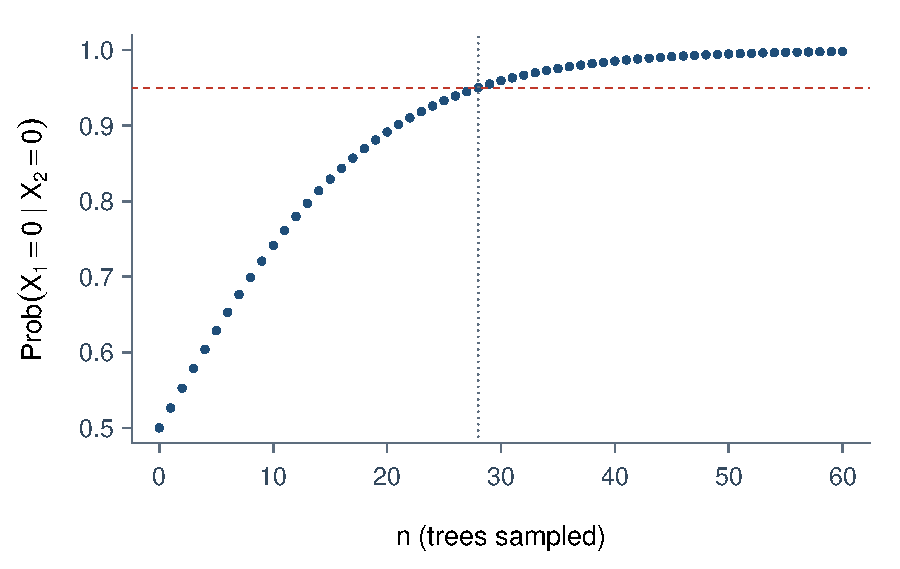
\includegraphics[width=0.68\linewidth]{ex15_occupancy.pdf}\end{center}

\begin{sanity}
$n=27$: $\frac1{1+0.9^{27}}=0.9450<0.95$; \ $n=28$: $0.9503\ge0.95$. \checkmark
\end{sanity}

\begin{answer}
(a) $1-\theta$ \quad (b) $1-\theta$ \quad (c) $1-\theta+\theta(1-\lambda)^n$ \quad (d) $\dfrac{1-\theta}{1-\theta+\theta(1-\lambda)^n}$ \quad (e) 1 \quad (f) 0 \quad (g) $(1-\lambda)^n$\\
(i) $\mathbf{n=28}$ trees with no detections.
\end{answer}

\begin{takeaway}
Absence of evidence becomes evidence of absence only gradually. Ignoring imperfect detection ($\lambda=1$) would let you declare absence after one empty sample.
\end{takeaway}

% ================================================================= Exercise 16
\exercise{1.16 --- Discovery rate of marine bivalve species}

\begin{problem}{16}
In a study that uses Bayesian methods to forecast the number of species that will be discovered in future years, [47] report that the number of marine bivalve species discovered each year from 2010-2015 was 64, 13, 33, 18, 30 and 20. Denoting $Y_t$ as the number of species discovered in year $t$ and assuming $Y_t|\lambda\iid\dist{Poisson}(\lambda)$ and $\lambda\sim\dist{Uniform}(0,100)$, plot the posterior distribution of $\lambda$.
\end{problem}

\begin{restate}
Six yearly counts come from a Poisson with unknown rate $\lambda$; with a flat prior on $(0,100)$, find and draw the posterior of $\lambda$.
\end{restate}

\begin{recall}
\begin{itemize}
\item Likelihood of independent observations = product of their PMFs.
\item $\dist{Gamma}(a,b)$ kernel: $\lambda^{a-1}e^{-b\lambda}$; mean $a/b$, SD $\sqrt a/b$.
\end{itemize}
\end{recall}

\begin{keyidea}
A flat prior is a constant, so the posterior has the shape of the likelihood (restricted to $0<\lambda<100$). Recognise the Gamma kernel.
\end{keyidea}

\solution
\step{Step 1 --- likelihood.}
\[
f(\mathbf y\mid\lambda)=\prod_{t=1}^6\frac{e^{-\lambda}\lambda^{y_t}}{y_t!}=\frac{e^{-6\lambda}\lambda^{\sum y_t}}{\prod y_t!}\ \propto\ \lambda^{178}e^{-6\lambda},
\]
because $\sum y_t=64+13+33+18+30+20=178$.
\why{Multiplying six factors $e^{-\lambda}$ gives $e^{-6\lambda}$; multiplying $\lambda^{y_1}\cdots\lambda^{y_6}$ adds the exponents.}

\step{Step 2 --- posterior.}
\[
p(\lambda\mid\mathbf y)\propto\lambda^{178}e^{-6\lambda}\cdot\frac{1}{100}\mathbb 1(0<\lambda<100)\ \propto\ \lambda^{179-1}e^{-6\lambda}\mathbb 1(0<\lambda<100),
\]
a $\dist{Gamma}(179,6)$ kernel cut off at 100. The cut-off is irrelevant: a $\dist{Gamma}(179,6)$ has probability $2\times10^{-91}$ above 100.

\step{Step 3 --- summaries.}
Mean $\frac{179}{6}=29.83$; SD $\frac{\sqrt{179}}{6}=2.23$; 95\% interval (\texttt{qgamma(c(.025,.975),179,6)}) $=(25.6,\ 34.4)$.
\begin{center}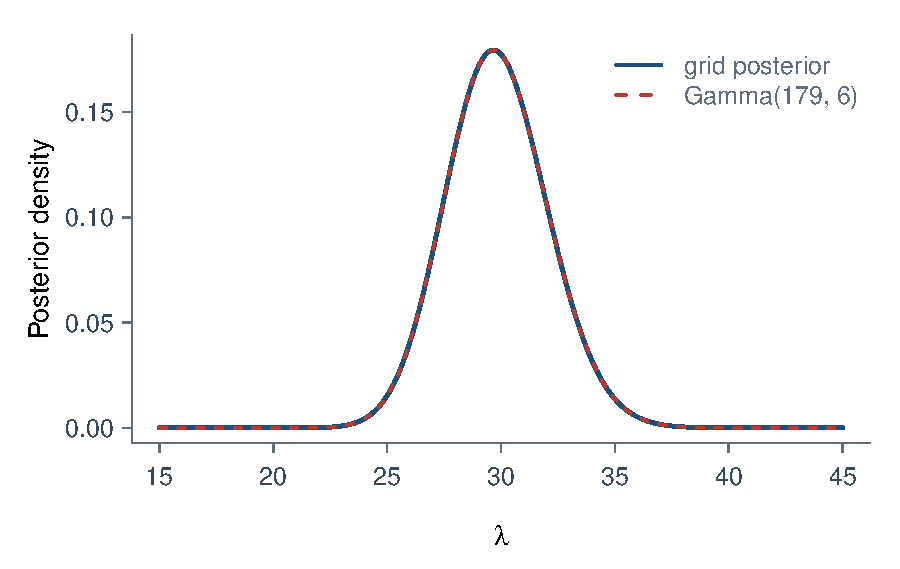
\includegraphics[width=0.7\linewidth]{ex16_lambda.pdf}\end{center}

\begin{sanity}
The grid-normalised posterior (solid) and the $\dist{Gamma}(179,6)$ density (dashed) coincide, and the posterior mean 29.8 is close to the sample mean $178/6=29.7$, as expected with a flat prior.
\end{sanity}

\begin{answer}
$\lambda\mid\mathbf y\sim\dist{Gamma}(179,\,6)$ (truncated at 100, negligibly): mean $\approx29.8$ species/year, 95\% interval $(25.6,\ 34.4)$.
\end{answer}

\begin{takeaway}
The yearly counts vary far more (SD $\approx18$) than a Poisson with mean 30 allows (SD $\approx5.5$): the Poisson model is too narrow here, so this interval is over-confident.
\end{takeaway}

% ================================================================= Exercise 17
\exercise{1.17 --- Posterior of a correlation coefficient}

\begin{problem}{17}
Assume that $(X,Y)$ follow the bivariate normal distribution and that both $X$ and $Y$ have marginal mean zero and marginal variance one. We observe six independent and identically distributed data points: $(-3.3,-2.6)$, $(0.1,-0.2)$, $(-1.1,-1.5)$, $(2.7,1.5)$, $(2.0,1.9)$ and $(-0.4,-0.3)$. Make a scatter plot of the data, and, assuming the correlation parameter $\rho$ has a $\dist{Uniform}(-1,1)$ prior, plot the posterior distribution of $\rho$.
\end{problem}

\begin{restate}
Six points from a standard bivariate normal with unknown correlation $\rho$; plot them, then find the posterior of $\rho$ with a flat prior.
\end{restate}

\begin{recall}
The joint density from Exercise 7 for one pair: $\dfrac{1}{2\pi\sqrt{1-\rho^2}}\exp\Big\{-\dfrac{x^2-2\rho xy+y^2}{2(1-\rho^2)}\Big\}$.
\end{recall}

\begin{keyidea}
One unknown $\Rightarrow$ \textbf{grid approximation}: evaluate the unnormalised posterior at thousands of $\rho$ values in $(-1,1)$ and divide by their sum (times the grid spacing).
\end{keyidea}

\solution
\step{Step 1 --- scatter plot.}
\begin{center}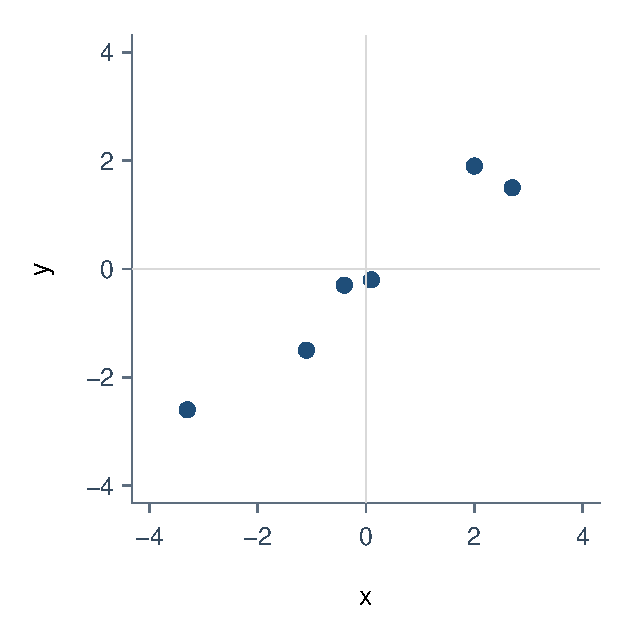
\includegraphics[width=0.42\linewidth]{ex17_scatter.pdf}\end{center}
The points lie close to a rising line: a strong positive association.

\step{Step 2 --- the likelihood.} Multiply the six densities; the exponents add:
\[
f(\text{data}\mid\rho)=\frac{1}{(2\pi)^6(1-\rho^2)^{3}}\exp\Big\{-\frac{S_{xx}-2\rho S_{xy}+S_{yy}}{2(1-\rho^2)}\Big\},
\]
where $S_{xx}=\sum x_i^2=23.56$, $S_{yy}=\sum y_i^2=15.00$, $S_{xy}=\sum x_iy_i=18.18$.
\why{$\big(\sqrt{1-\rho^2}\big)^6=(1-\rho^2)^3$, and $\sum(x_i^2-2\rho x_iy_i+y_i^2)=S_{xx}-2\rho S_{xy}+S_{yy}$.}

\step{Step 3 --- log posterior on a grid.}
With the flat prior,
\[
\log p(\rho\mid\text{data})=-3\log(1-\rho^2)-\frac{S_{xx}-2\rho S_{xy}+S_{yy}}{2(1-\rho^2)}+\text{const}.
\]
\begin{lstlisting}
rg   <- seq(-0.999, 0.999, length.out = 3999)
ll   <- -3*log(1 - rg^2) - (Sxx - 2*rg*Sxy + Syy) / (2*(1 - rg^2))
post <- exp(ll - max(ll))                    # subtract max to avoid underflow
post <- post / sum(post * diff(rg)[1])       # normalise to area 1
\end{lstlisting}
\begin{center}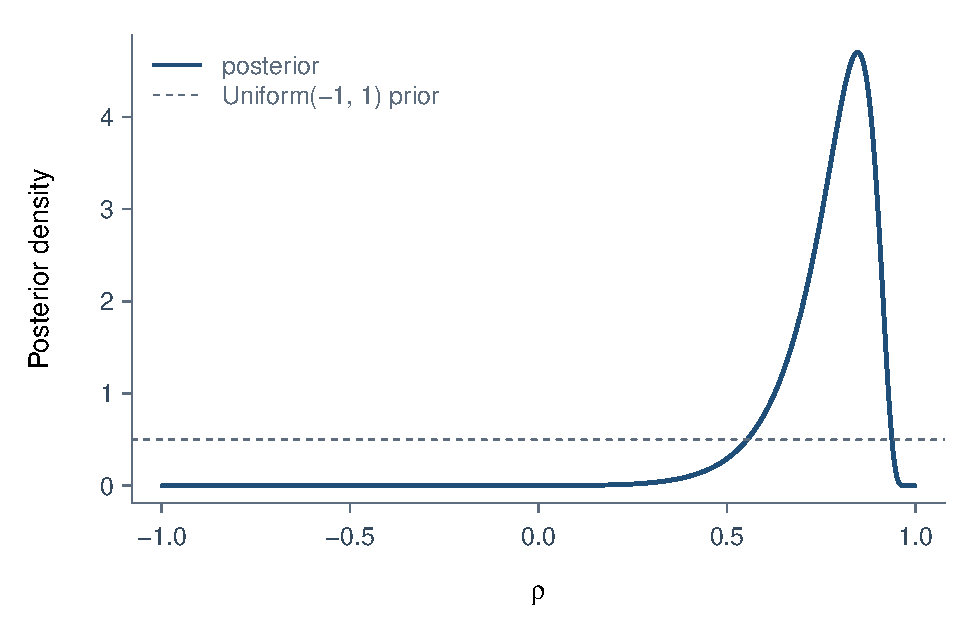
\includegraphics[width=0.7\linewidth]{ex17_rho.pdf}\end{center}

\step{Step 4 --- summaries.}
Mode $0.85$, mean $0.78$, 95\% interval $(0.49,\ 0.92)$; $\Prob(\rho>0\mid\text{data})\approx1$.

\begin{sanity}
Why is the posterior centred below the sample correlation (0.97)? Because the variances are \emph{known} to be 1, so $\V(X-Y)=2(1-\rho)$. The data give $\frac16\sum(x_i-y_i)^2=\frac{S_{xx}+S_{yy}-2S_{xy}}{6}=0.37$, which matches $2(1-\rho)$ for $\rho\approx0.82$ --- right where the posterior sits.
\end{sanity}

\begin{answer}
Posterior of $\rho$ concentrated on strong positive values: mode $\approx0.85$, mean $\approx0.78$, 95\% interval $\approx(0.49,\ 0.92)$.
\end{answer}

\begin{takeaway}
With $n=6$ the posterior is wide and skewed --- report the whole distribution, not just a point estimate.
\end{takeaway}

% ================================================================= Exercise 18
\exercise{1.18 --- Classifying deforestation from NDVI}

\begin{problem}{18}
The normalized difference vegetation index (NDVI) is commonly used to classify land cover using remote sensing data. Hypothetically, say that NDVI follows a $\dist{Beta}(25,10)$ distribution for pixels in a rain forest, and a $\dist{Beta}(10,15)$ distribution for pixels in a deforested area now used for agriculture. Assuming about 10\% of the rain forest has been deforested, your objective is to build a rule to classify individual pixels as deforested based on their NDVI.
\begin{enumerate}[(a)]
\item Plot the PDF of NDVI for forested and deforested pixels, and the marginal distribution of NDVI averaging over categories.
\item Give an expression for the probability that a pixel is deforested given its NDVI value, and plot this probability by NDVI.
\item You will classify a pixel as deforested if you are at least 90\% sure it is deforested. Following this rule, give the range of NDVI that will lead to a pixel being classified as deforested.
\end{enumerate}
\end{problem}

\begin{restate}
Forest pixels have high NDVI, deforested pixels lower NDVI, and only 10\% are deforested. For a given NDVI, how likely is deforestation, and which NDVI values give at least 90\% certainty?
\end{restate}

\begin{recall}
$\dist{Beta}(a,b)$ density: $\frac{x^{a-1}(1-x)^{b-1}}{B(a,b)}$ on $(0,1)$, mean $\frac a{a+b}$. Bayes' rule with a continuous observation uses densities (Exercise 11).
\end{recall}

\begin{keyidea}
A two-class Bayes classifier: prior (0.1 deforested, 0.9 forest) $\times$ class density, normalised. The marginal density of NDVI is the mixture $0.9f_F+0.1f_D$.
\end{keyidea}

\solution
\step{(a) Densities.}
Forest $\dist{Beta}(25,10)$ has mean $\frac{25}{35}=0.71$; deforested $\dist{Beta}(10,15)$ has mean $\frac{10}{25}=0.40$.
\begin{center}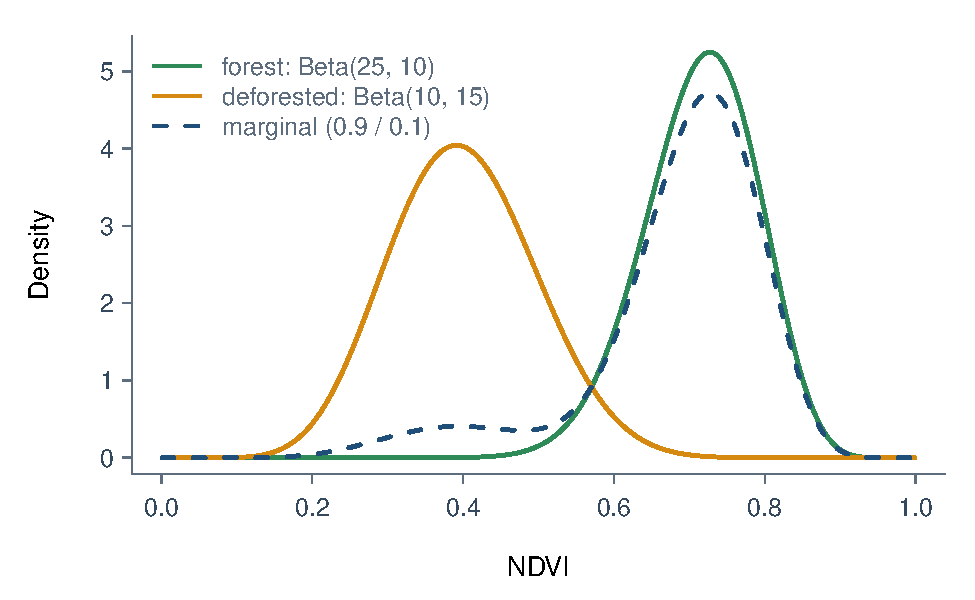
\includegraphics[width=0.75\linewidth]{ex18_densities.pdf}\end{center}
The marginal (dashed) is mostly the forest curve, with a small shoulder at low NDVI from deforested pixels.

\step{(b) Posterior probability of deforestation.}
\[
\Prob(D\mid x)=\frac{0.1\,f_D(x)}{0.1\,f_D(x)+0.9\,f_F(x)}=\frac{1}{1+9\,\frac{f_F(x)}{f_D(x)}}.
\]
\why{Divide numerator and denominator by $0.1f_D(x)$.}
The density ratio simplifies:
\[
\frac{f_F(x)}{f_D(x)}=\frac{x^{24}(1-x)^{9}/B(25,10)}{x^{9}(1-x)^{14}/B(10,15)}=\frac{B(10,15)}{B(25,10)}\cdot\frac{x^{15}}{(1-x)^5},
\]
which increases with $x$. So $\Prob(D\mid x)$ \emph{decreases} as NDVI increases.
\begin{center}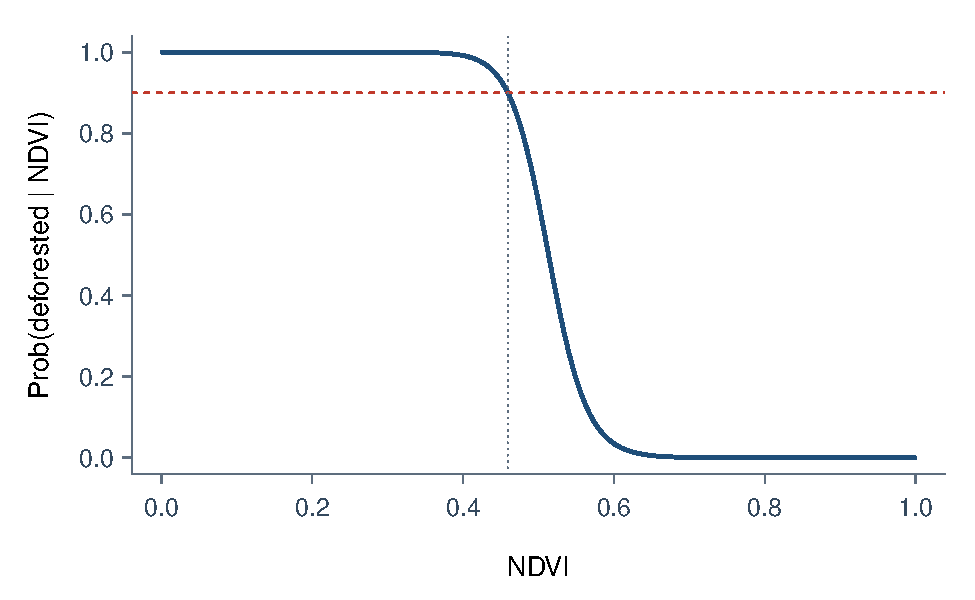
\includegraphics[width=0.75\linewidth]{ex18_prob.pdf}\end{center}

\step{(c) The 90\% rule.}
Because $\Prob(D\mid x)$ is decreasing, ``$\Prob(D\mid x)\ge0.9$'' is the same as ``$x\le c$'' where $\Prob(D\mid c)=0.9$. Solving numerically (\texttt{uniroot}): $c=0.459$.

\begin{sanity}
At the cut-off, $\Prob(D\mid0.459)=0.900$ by construction. Error rates: only 0.1\% of forest pixels fall below 0.459 (few false alarms); 73\% of deforested pixels do.
\end{sanity}

\begin{answer}
(b) $\Prob(D\mid x)=\dfrac{0.1\,\dist{Beta}(x;10,15)}{0.1\,\dist{Beta}(x;10,15)+0.9\,\dist{Beta}(x;25,10)}$.\\
(c) Classify as deforested when $\mathbf{NDVI<0.459}$.
\end{answer}

\begin{takeaway}
Requiring 90\% certainty when only 10\% of pixels are deforested is strict: 27\% of deforested pixels are missed.
\end{takeaway}

% ================================================================= Exercise 19
\exercise{1.19 --- How many customers came?}

\begin{problem}{19}
Let $n$ be the unknown number of customers who visit a store on the day of a sale. The number of customers who make a purchase is $Y|n\sim\dist{Binomial}(n,\theta)$ where $\theta$ is the known probability of making a purchase given the customer visited the store. The prior is $n\sim\dist{Poisson}(5)$. Assuming $\theta$ is known and $n$ is the unknown parameter, plot the posterior distribution of $n$ for all combinations of $Y\in\{0,5,10\}$ and $\theta\in\{0.2,0.5\}$, and comment on the effect of $Y$ and $\theta$ on the posterior.
\end{problem}

\begin{restate}
We only see the number of buyers $Y$. Infer the number of visitors $n$, knowing each visitor buys with probability $\theta$.
\end{restate}

\begin{recall}
$\binom nY=\frac{n!}{Y!(n-Y)!}$. A function of $k$ proportional to $\frac{\mu^k}{k!}$ is a $\dist{Poisson}(\mu)$ kernel.
\end{recall}

\begin{keyidea}
The unknown $n$ is discrete, so the posterior is a PMF on $n=Y,Y+1,\dots$ (we need $n\ge Y$). The $n!$'s cancel and a Poisson kernel in $n-Y$ appears.
\end{keyidea}

\solution
\step{Step 1 --- prior $\times$ likelihood} (for $n\ge Y$):
\[
p(n\mid Y)\propto\underbrace{\frac{e^{-5}5^n}{n!}}_{\text{prior}}\ \underbrace{\frac{n!}{Y!(n-Y)!}\theta^Y(1-\theta)^{n-Y}}_{\text{likelihood}}.
\]
\step{Step 2 --- cancel and drop constants.}
The $n!$ cancels; $e^{-5}$, $Y!$ and $\theta^Y$ do not involve $n$:
\[
p(n\mid Y)\propto\frac{5^n(1-\theta)^{n-Y}}{(n-Y)!}=5^Y\cdot\frac{5^{n-Y}(1-\theta)^{n-Y}}{(n-Y)!}\propto\frac{[5(1-\theta)]^{n-Y}}{(n-Y)!}.
\]
\why{$5^n=5^Y\cdot5^{n-Y}$, and $5^Y$ is a constant.}
\step{Step 3 --- recognise it.}
With $m=n-Y$, this is $\frac{\mu^m}{m!}$ with $\mu=5(1-\theta)$: a Poisson kernel. Hence
\[
n\mid Y\ =\ Y+M,\qquad M\sim\dist{Poisson}\big(5(1-\theta)\big).
\]
In words: the $Y$ buyers certainly came; the number of \emph{non-buyers} is Poisson with mean $5(1-\theta)$.

\step{Step 4 --- summaries and plot.}
$\E(n\mid Y)=Y+5(1-\theta)$, $\V(n\mid Y)=5(1-\theta)$. For $\theta=0.2$: means 4, 9, 14 (SD 2.0); for $\theta=0.5$: means 2.5, 7.5, 12.5 (SD 1.58).
\begin{center}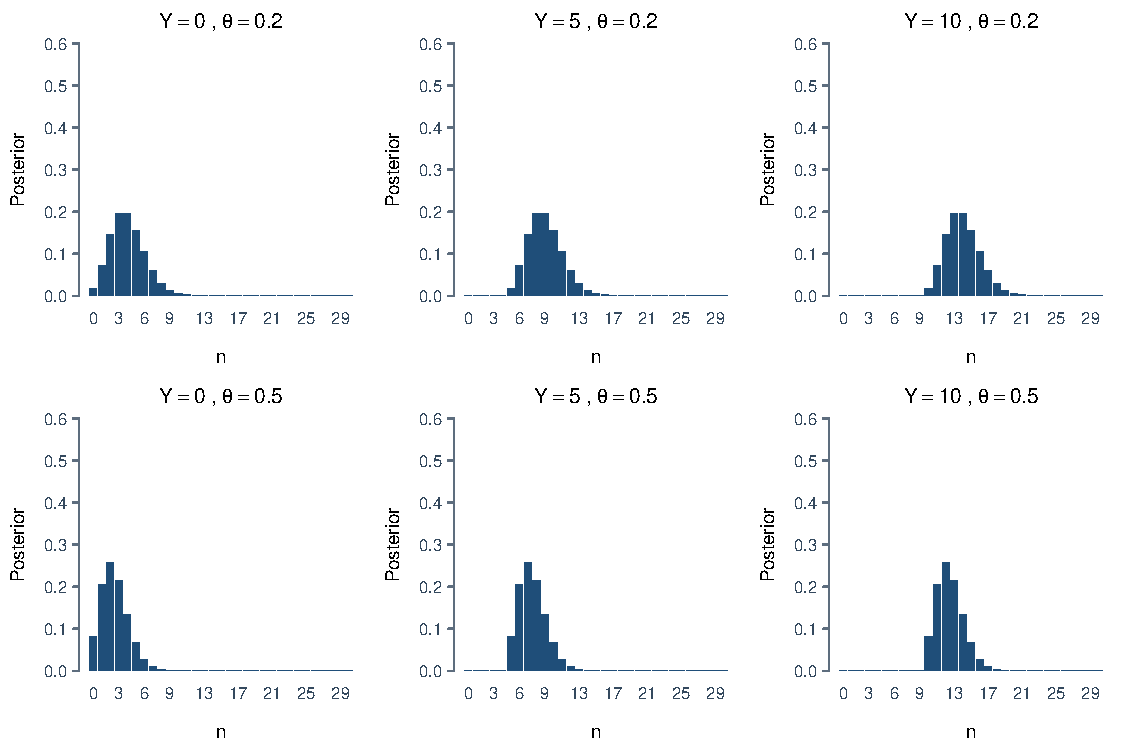
\includegraphics[width=0.95\linewidth]{ex19_customers.pdf}\end{center}

\step{Step 5 --- comments.}
\begin{itemize}
\item \textbf{$Y$} only \emph{shifts} the posterior; its shape is the same for $Y=0,5,10$. $Y=10$ pushes $n$ far above the prior mean 5, because $n\ge Y$ is a hard constraint.
\item \textbf{$\theta$}: larger $\theta$ means fewer hidden non-buyers, so the posterior is narrower and closer to $Y$.
\item $Y=0$ shifts the posterior \emph{down} from the prior: no buyers suggests fewer visitors.
\end{itemize}

\begin{sanity}
Brute-force normalisation of $\text{prior}\times\text{likelihood}$ over $n=0,\dots,30$ in \texttt{ch01.R} gives exactly these means and SDs. \checkmark
\end{sanity}

\begin{answer}
$n\mid Y\sim Y+\dist{Poisson}(5(1-\theta))$. $Y$ shifts the posterior right; larger $\theta$ makes it narrower and closer to $Y$.
\end{answer}

\begin{takeaway}
Remember the support restriction $n\ge Y$; forgetting it puts probability on impossible values.
\end{takeaway}

% ================================================================= Exercise 20
\exercise{1.20 --- Seedling survival: the beta--binomial model}

\begin{problem}{20}
Last spring your lab planted ten seedlings, and two survived the winter. Let $\theta$ be the probability that a seedling survives the winter.
\begin{enumerate}[(a)]
\item Assuming a uniform prior distribution for $\theta$, compute its posterior mean and standard deviation.
\item Assuming the same prior as in (a), compute and compare the equal-tailed and highest density 95\% posterior credible intervals.
\item If you plant another 10 seedlings next year, what is the posterior predictive probability that at least one will survive the winter?
\end{enumerate}
\end{problem}

\begin{restate}
2 of 10 seedlings survived. With a flat prior on the survival probability, summarise the posterior, give two kinds of 95\% intervals, and predict next year.
\end{restate}

\begin{recall}
\begin{itemize}
\item $\dist{Beta}(a,b)$: mean $\frac{a}{a+b}$, variance $\frac{ab}{(a+b)^2(a+b+1)}$.
\item $B(a,b)=\int_0^1t^{a-1}(1-t)^{b-1}\dd t=\frac{\Gamma(a)\Gamma(b)}{\Gamma(a+b)}$, and $\Gamma(k)=(k-1)!$ for integers.
\item \textbf{Equal-tailed} interval: cut 2.5\% from each tail. \textbf{HPD} interval: the \emph{shortest} interval with 95\% probability (density equal at both ends).
\end{itemize}
\end{recall}

\begin{keyidea}
Uniform $=\dist{Beta}(1,1)$ prior + binomial data $\Rightarrow\dist{Beta}(1+Y,\ 1+n-Y)$ posterior. For prediction, \emph{average} $(1-\theta)^{10}$ over the posterior instead of plugging in one value of $\theta$.
\end{keyidea}

\solution
\step{Step 1 --- posterior.}
\[
p(\theta\mid Y)\propto\underbrace{\theta^2(1-\theta)^8}_{\text{likelihood}}\cdot\underbrace{1}_{\text{prior}}=\theta^{3-1}(1-\theta)^{9-1}\ \Rightarrow\ \theta\mid Y\sim\dist{Beta}(3,9).
\]
\step{(a) Mean and SD.}
\[
\E(\theta\mid Y)=\frac{3}{3+9}=0.25,\qquad\V=\frac{3\cdot9}{12^2\cdot13}=\frac{27}{1872}=0.01442,\qquad\text{SD}=0.120.
\]
\step{(b) Equal-tailed interval.} \texttt{qbeta(c(.025,.975),3,9)} $=(0.060,\ 0.518)$, width 0.458.
\step{(b) HPD interval.} For each lower end $\ell$ the matching upper end is $u=F^{-1}(F(\ell)+0.95)$; minimise $u-\ell$ over $\ell$ (\texttt{optimize}): HPD $=(0.041,\ 0.484)$, width 0.443.
\begin{center}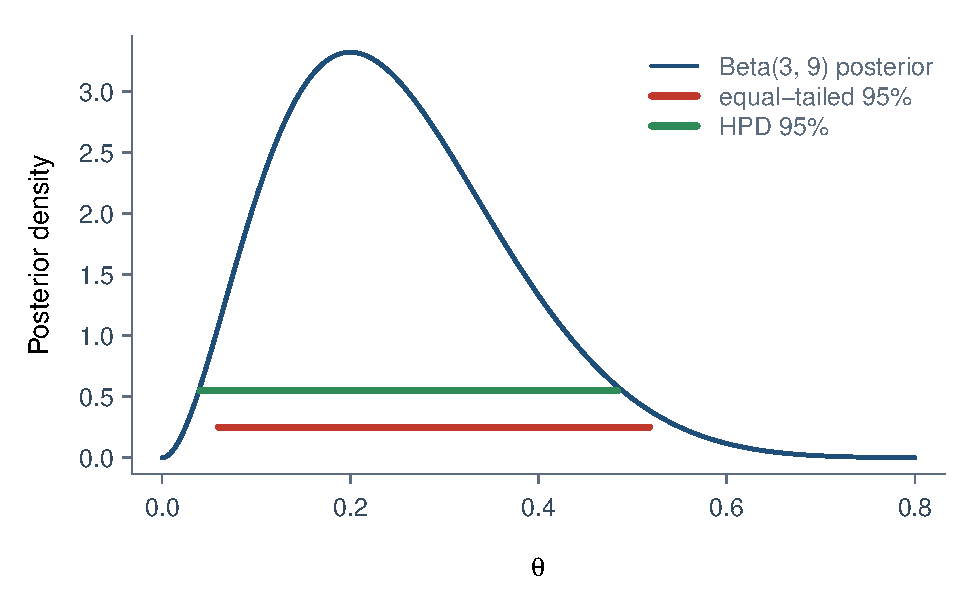
\includegraphics[width=0.72\linewidth]{ex20_intervals.pdf}\end{center}
The posterior is right-skewed (mode 0.2), so the HPD interval is shifted \emph{left} and is about 3\% shorter.

\step{(c) Posterior predictive.}
Let $Y^*$ be next year's survivors out of 10. Given $\theta$, $\Prob(Y^*=0\mid\theta)=(1-\theta)^{10}$. Averaging over the posterior:
\[
\Prob(Y^*=0\mid Y)=\int_0^1(1-\theta)^{10}\frac{\theta^2(1-\theta)^8}{B(3,9)}\dd\theta=\frac{1}{B(3,9)}\int_0^1\theta^2(1-\theta)^{18}\dd\theta=\frac{B(3,19)}{B(3,9)}.
\]
With factorials:
\[
\frac{B(3,19)}{B(3,9)}=\frac{\Gamma(3)\Gamma(19)/\Gamma(22)}{\Gamma(3)\Gamma(9)/\Gamma(12)}=\frac{18!\,11!}{21!\,8!}=\frac{11\cdot10\cdot9}{21\cdot20\cdot19}=\frac{990}{7980}=0.1241.
\]
\why{$\frac{18!}{21!}=\frac{1}{21\cdot20\cdot19}$ and $\frac{11!}{8!}=11\cdot10\cdot9$.}
So $\Prob(Y^*\ge1\mid Y)=1-0.1241=0.876$.

\begin{sanity}
HPD check: the posterior density is the same at both ends of the HPD interval (0.585), as it must be. Simulation check of (c): draw $\theta\sim\dist{Beta}(3,9)$, then $Y^*\sim\dist{Bin}(10,\theta)$; the fraction with $Y^*\ge1$ is 0.876.
\end{sanity}

\begin{answer}
(a) $\theta\mid Y\sim\dist{Beta}(3,9)$: mean $0.25$, SD $0.120$.\\
(b) Equal-tailed $(0.060,0.518)$; HPD $(0.041,0.484)$ --- shorter and shifted toward 0 because of the right skew.\\
(c) $1-\frac{990}{7980}=\mathbf{0.876}$.
\end{answer}

\begin{takeaway}
Plugging in $\hat\theta=0.25$ gives $1-0.75^{10}=0.944$ --- too optimistic, because it ignores the real chance that $\theta$ is small.
\end{takeaway}

% ================================================================= Exercise 21
\exercise{1.21 --- Machine part failures (AND/OR systems)}

\begin{problem}{21}
$X_1$ and $X_2$ are binary indicators of failure for two parts of a machine. Independent tests have shown that $X_1\sim\dist{Bernoulli}(1/2)$ and $X_2\sim\dist{Bernoulli}(1/3)$. $Y_1$ and $Y_2$ are binary indicators of two system failures. We know that $Y_1=1$ if both $X_1=1$ and $X_2=1$ and $Y_1=0$ otherwise, and $Y_2=0$ if both $X_1=0$ and $X_2=0$ and $Y_2=1$ otherwise. Compute the following probabilities:
\begin{enumerate}[(a)]
\item The probability that $X_1=1$ and $X_2=1$ given $Y_1=1$.
\item The probability that $X_1=1$ and $X_2=1$ given $Y_2=1$.
\item The probability that $X_1=1$ given $Y_1=1$.
\item The probability that $X_1=1$ given $Y_2=1$.
\end{enumerate}
\end{problem}

\begin{restate}
$Y_1$ = ``both parts failed'' (AND). $Y_2$ = ``at least one part failed'' (OR). What does each system failure tell us about the parts?
\end{restate}

\begin{recall}
For independent events, $\Prob(A\cap B)=\Prob(A)\Prob(B)$. Conditional probability: $\Prob(A\mid B)=\Prob(A\cap B)/\Prob(B)$.
\end{recall}

\begin{keyidea}
List all four $(x_1,x_2)$ combinations with their probabilities and the resulting $Y_1,Y_2$. Then every answer is ``add the qualifying rows, divide by the rows of the condition''.
\end{keyidea}

\solution
\step{Step 1 --- the full table.}
\begin{center}
\begin{tabular}{cc|c|cc}\toprule
$x_1$ & $x_2$ & probability & $Y_1$ (AND) & $Y_2$ (OR)\\\midrule
0&0&$\frac12\cdot\frac23=\frac13$&0&0\\
1&0&$\frac12\cdot\frac23=\frac13$&0&1\\
0&1&$\frac12\cdot\frac13=\frac16$&0&1\\
1&1&$\frac12\cdot\frac13=\frac16$&1&1\\\bottomrule
\end{tabular}
\end{center}
So $\Prob(Y_1=1)=\frac16$ (last row) and $\Prob(Y_2=1)=\frac13+\frac16+\frac16=\frac23$.

\step{(a)} Rows with $Y_1=1$: only $(1,1)$. $\Prob(X_1=X_2=1\mid Y_1=1)=\frac{1/6}{1/6}=\mathbf1$.
\step{(b)} Rows with $Y_2=1$: the last three (total $\frac23$); of these, $(1,1)$ has $\frac16$. Answer $\frac{1/6}{2/3}=\mathbf{\frac14}$.
\step{(c)} $Y_1=1$ forces $X_1=1$: $\mathbf1$.
\step{(d)} Among the $Y_2=1$ rows, those with $x_1=1$ are $(1,0)$ and $(1,1)$: $\frac13+\frac16=\frac12$. Answer $\frac{1/2}{2/3}=\mathbf{\frac34}$.

\begin{sanity}
In (d) the probability rises from the prior $\frac12$ to $\frac34$: learning that \emph{something} failed makes each part more suspect. \checkmark
\end{sanity}

\begin{answer}
(a) 1 \qquad (b) $1/4$ \qquad (c) 1 \qquad (d) $3/4$
\end{answer}

\begin{takeaway}
Given $Y_2=1$ the parts become dependent (``explaining away''): if we then learn $X_2=1$, the probability that $X_1=1$ drops back to $\frac12$.
\end{takeaway}

% ================================================================= Exercise 22
\exercise{1.22 --- Clutch free throws in the NBA}

\begin{problem}{22}
The table below has the overall free throw proportion and results of free throws taken in pressure situations, defined as ``clutch'' (https://stats.nba.com/), for ten National Basketball Association players (those who received the most votes for the Most Valuable Player Award) for the 2016--2017 season. Since the overall proportion is computed using a large sample size, assume it is fixed, and analyze the clutch data for each player separately using Bayesian methods. Assume a uniform prior throughout this problem.
\begin{center}
\small
\begin{tabular}{lccc}\toprule
Player & Overall proportion & Clutch makes & Clutch attempts\\\midrule
Russell Westbrook & 0.845 & 64 & 75\\
James Harden & 0.847 & 72 & 95\\
Kawhi Leonard & 0.880 & 55 & 63\\
LeBron James & 0.674 & 27 & 39\\
Isaiah Thomas & 0.909 & 75 & 83\\
Stephen Curry & 0.898 & 24 & 26\\
Giannis Antetokounmpo & 0.770 & 28 & 41\\
John Wall & 0.801 & 66 & 82\\
Anthony Davis & 0.802 & 40 & 54\\
Kevin Durant & 0.875 & 13 & 16\\\bottomrule
\end{tabular}
\end{center}
\begin{enumerate}[(a)]
\item Describe your model for studying the clutch success probability including the likelihood and prior.
\item Plot the posteriors of the clutch success probabilities.
\item Summarize the posteriors in a table.
\item Do you find evidence that any of the players have a different clutch percentage than overall percentage?
\item Are the results sensitive to your prior? That is, do small changes in the prior lead to substantial changes in the posterior?
\end{enumerate}
\end{problem}

\begin{restate}
For each player, estimate the probability of making a free throw under pressure and compare it with their (known) overall percentage.
\end{restate}

\begin{recall}
Beta--binomial update: $Y\mid\theta\sim\dist{Binomial}(n,\theta)$, $\theta\sim\dist{Beta}(a,b)$ $\Rightarrow$ $\theta\mid Y\sim\dist{Beta}(a+Y,\ b+n-Y)$. Uniform $=\dist{Beta}(1,1)$.
\end{recall}

\begin{keyidea}
The key number for (d) is $\Prob(\theta_i<q_i\mid Y_i)$ (posterior probability that player $i$ is worse in the clutch). Near 0.5 $\Rightarrow$ no evidence; near 0 or 1 $\Rightarrow$ evidence of a difference.
\end{keyidea}

\solution
\step{(a) Model.}
\[
Y_i\mid\theta_i\sim\dist{Binomial}(n_i,\theta_i),\qquad\theta_i\sim\dist{Beta}(1,1)
\quad\Longrightarrow\quad\theta_i\mid Y_i\sim\dist{Beta}(Y_i+1,\,n_i-Y_i+1).
\]
This assumes clutch shots are independent with a constant success probability per player. Example: Westbrook $\Rightarrow\dist{Beta}(65,12)$.

\step{(b) Posteriors} (red dashed line: overall proportion $q_i$):
\begin{center}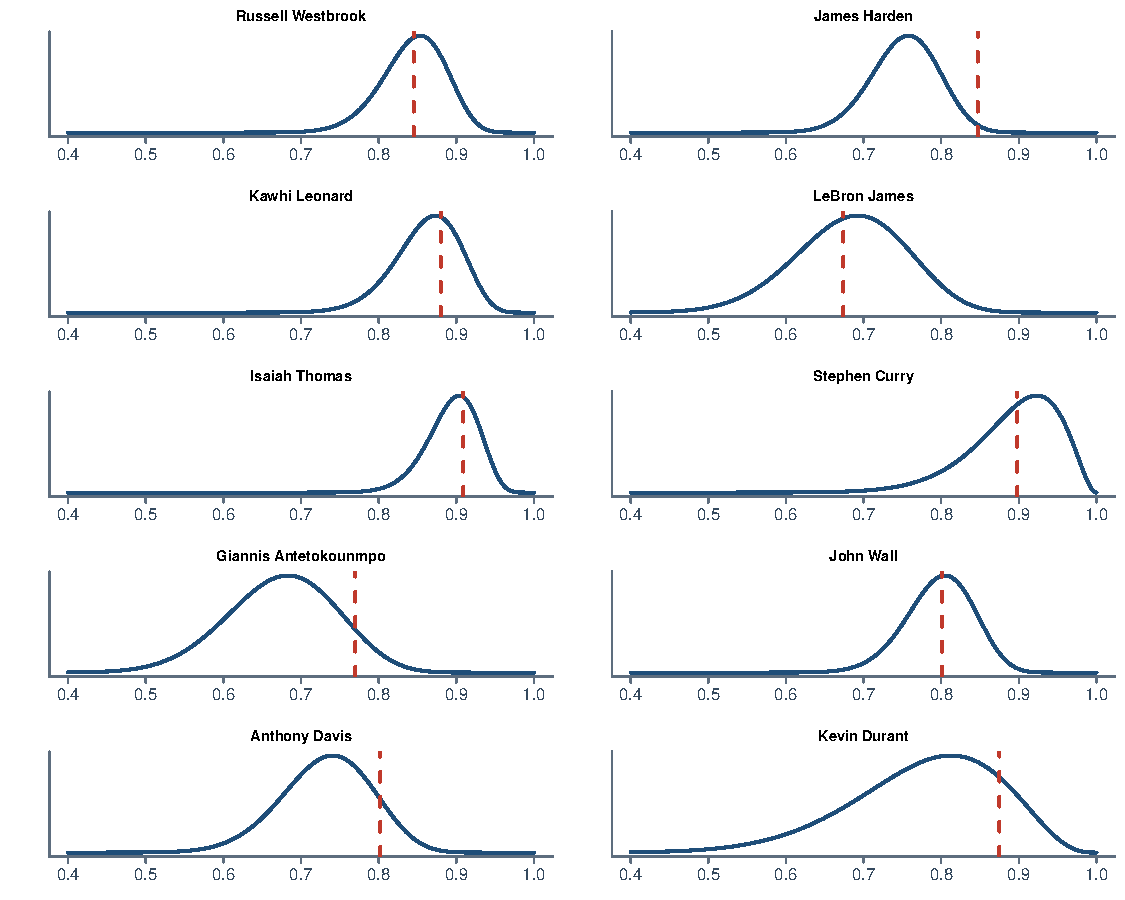
\includegraphics[width=0.92\linewidth]{ex22_clutch.pdf}\end{center}

\step{(c) Summary table.}
\begin{center}
\small
\begin{tabular}{lcccc}\toprule
Player & Overall $q_i$ & Posterior mean & 95\% interval & $\Prob(\theta_i<q_i\mid Y_i)$\\\midrule
Russell Westbrook & 0.845 & 0.844 & (0.756, 0.916) & 0.479\\
James Harden & 0.847 & 0.753 & (0.663, 0.833) & \textbf{0.991}\\
Kawhi Leonard & 0.880 & 0.862 & (0.768, 0.934) & 0.640\\
LeBron James & 0.674 & 0.683 & (0.535, 0.814) & 0.435\\
Isaiah Thomas & 0.909 & 0.894 & (0.821, 0.950) & 0.645\\
Stephen Curry & 0.898 & 0.893 & (0.757, 0.976) & 0.471\\
Giannis Antetokounmpo & 0.770 & 0.674 & (0.529, 0.804) & \textbf{0.917}\\
John Wall & 0.801 & 0.798 & (0.706, 0.876) & 0.509\\
Anthony Davis & 0.802 & 0.732 & (0.610, 0.839) & 0.887\\
Kevin Durant & 0.875 & 0.778 & (0.566, 0.932) & 0.846\\\bottomrule
\end{tabular}
\end{center}
\why{Posterior mean $=\frac{Y_i+1}{n_i+2}$; e.g.\ Harden: $\frac{73}{97}=0.753$. The last column is \texttt{pbeta(q, Y+1, n-Y+1)}.}

\step{(d) Evidence of a clutch effect?}
\begin{itemize}
\item \textbf{Harden}: $\Prob(\theta<q)=0.991$ and his 95\% interval $(0.663,0.833)$ excludes $0.847$: strong evidence he shoots \emph{worse} in the clutch.
\item \textbf{Antetokounmpo} (0.917) and \textbf{Davis} (0.887): moderate evidence, but $q$ lies inside their intervals.
\item Everyone else: probabilities near 0.5 --- no evidence. Nobody shows evidence of being \emph{better} in the clutch.
\end{itemize}

\step{(e) Prior sensitivity.} Re-run with Jeffreys $\dist{Beta}(\frac12,\frac12)$ and $\dist{Beta}(2,2)$:
\begin{center}
\small
\begin{tabular}{lccc}\toprule
Player & Uniform & Jeffreys & Beta(2,2)\\\midrule
Westbrook & 0.479 & 0.435 & 0.565\\
Harden & 0.991 & 0.989 & 0.994\\
Leonard & 0.640 & 0.586 & 0.735\\
James & 0.435 & 0.411 & 0.483\\
Thomas & 0.645 & 0.588 & 0.745\\
Curry & 0.471 & 0.366 & 0.657\\
Antetokounmpo & 0.917 & 0.904 & 0.937\\
Wall & 0.509 & 0.476 & 0.574\\
Davis & 0.887 & 0.869 & 0.915\\
Durant & 0.846 & 0.788 & 0.921\\\bottomrule
\end{tabular}
\end{center}
The conclusions do not change; numbers move most for players with few attempts (Curry $n=26$, Durant $n=16$).

\begin{answer}
(a) $Y_i|\theta_i\sim\dist{Bin}(n_i,\theta_i)$, $\theta_i\sim\dist{Beta}(1,1)\Rightarrow\dist{Beta}(Y_i+1,n_i-Y_i+1)$. (b),(c) Figure and table. (d) Strong evidence only for Harden (worse); moderate for Antetokounmpo and Davis. (e) Conclusions robust to small prior changes.
\end{answer}

\begin{takeaway}
With ten players, one looking unusual is not surprising (multiple comparisons). Chapter 3, Exercise 7 revisits this with a model that shares information across players.
\end{takeaway}

% ================================================================= Exercise 23
\exercise{1.23 --- Who wrote the disputed Federalist Papers?}

\begin{problem}{23}
In the early twentieth century, it was generally agreed that Hamilton and Madison (ignore Jay for now) wrote 51 and 14 Federalist Papers, respectively. There was dispute over how to attribute 12 other papers between these two authors. In the 51 papers attributed to Hamilton, the word ``upon'' was used 3.24 times per 1,000 words, compared to 0.23 times per 1,000 words in the 14 papers attributed to Madison (for historical perspective on this problem, see [110]).
\begin{enumerate}[(a)]
\item If the word ``upon'' is used three times in a disputed text of length 1,000 words and we assume the prior probability 0.5, what is the posterior probability the paper was written by Hamilton?
\item Give one assumption you are making in (a) that is likely unreasonable. Justify your answer.
\item In (a), if we changed the number of instances of ``upon'' to one, do you expect the posterior probability to increase, decrease or stay the same? Why?
\item In (a), if we changed the text length to 10,000 words and number of instances of ``upon'' to 30, do you expect the posterior probability to increase, decrease or stay the same? Why?
\item Let $Y$ be the number of observed number of instances of ``upon'' in 1,000 words. Compute the posterior probability the paper was written by Hamilton for each $Y\in\{0,1,\dots,20\}$, plot these posterior probabilities versus $Y$ and give a rule for the number of instances of ``upon'' needed before the paper should be attributed to Hamilton.
\end{enumerate}
\end{problem}

\begin{restate}
Hamilton writes ``upon'' often; Madison rarely. Use how often it appears in a disputed paper to decide who wrote it.
\end{restate}

\begin{recall}
\begin{itemize}
\item \textbf{Odds form of Bayes' rule}: posterior odds $=$ prior odds $\times$ likelihood ratio:
$\dfrac{\Prob(H\mid Y)}{\Prob(M\mid Y)}=\dfrac{\Prob(H)}{\Prob(M)}\cdot\dfrac{f(Y\mid H)}{f(Y\mid M)}$, and probability $=\frac{\text{odds}}{1+\text{odds}}$.
\item Word counts in a text of $L$ thousand words: $Y\sim\dist{Poisson}(\text{rate}\times L)$.
\end{itemize}
\end{recall}

\begin{keyidea}
With prior odds 1, the posterior odds are just the likelihood ratio $\frac{\dist{Poisson}(y;\,3.24L)}{\dist{Poisson}(y;\,0.23L)}$.
\end{keyidea}

\solution
\step{Step 1 --- the likelihood ratio in general.}
\[
\frac{f(y\mid H)}{f(y\mid M)}=\frac{e^{-3.24L}(3.24L)^y/y!}{e^{-0.23L}(0.23L)^y/y!}=e^{-(3.24-0.23)L}\Big(\frac{3.24}{0.23}\Big)^y=e^{-3.01L}\,(14.087)^y.
\]
\why{The $y!$ and $L^y$ cancel; $e^{-3.24L}/e^{-0.23L}=e^{-3.01L}$.}

\step{(a) $y=3$, $L=1$.}
$e^{-3.01}=0.04929$ and $14.087^3=2795.5$, so the likelihood ratio is $0.04929\times2795.5=137.8$. With prior odds 1:
\[
\Prob(H\mid Y=3)=\frac{137.8}{1+137.8}=\mathbf{0.993}.
\]
\step{(b) An unreasonable assumption.}
The Poisson model assumes each ``upon'' occurs independently at a constant rate. Real word use depends on topic and style, so occurrences cluster and counts are \emph{over-dispersed} (variance $>$ mean). Also, 3.24 and 0.23 are treated as exactly known, though they are estimates.

\step{(c) $y=1$: decrease.}
One ``upon'' is typical of Madison (expected 0.23) and unusually low for Hamilton (expected 3.24). Likelihood ratio $=0.04929\times14.087=0.694<1$, so $\Prob(H\mid Y=1)=\frac{0.694}{1.694}=0.410$.

\step{(d) $L=10$, $y=30$: increase.}
Same rate as (a) but ten times more text = ten times more evidence. $\log\text{LR}=-30.1+30\log14.087=-30.1+79.4=49.3$, so the odds are $e^{49.3}\approx2.6\times10^{21}$ and the probability is essentially 1.

\step{(e) The whole curve.}
\begin{center}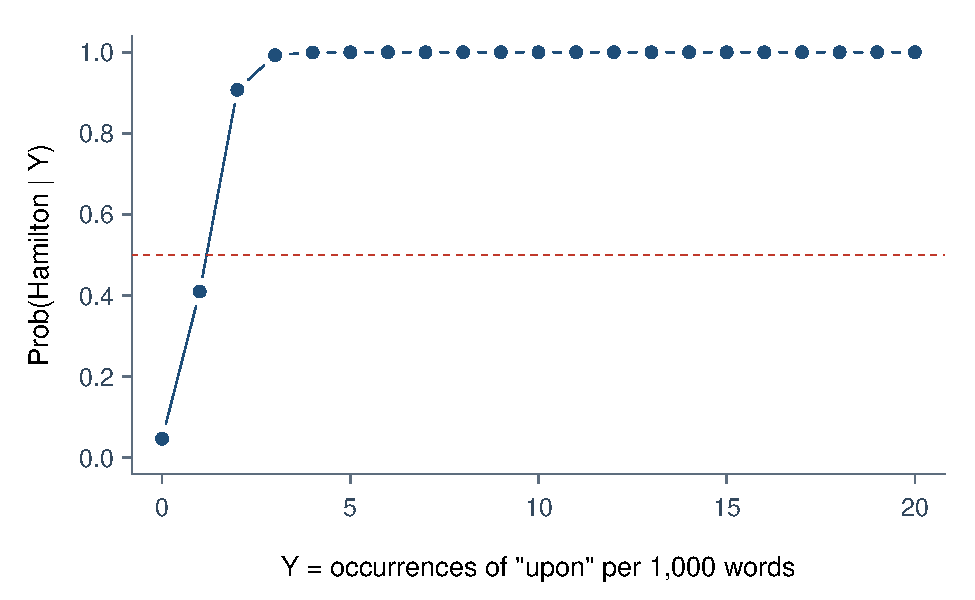
\includegraphics[width=0.72\linewidth]{ex23_federalist.pdf}\end{center}
\begin{center}
\small
\begin{tabular}{c|cccccc}\toprule
$Y$ & 0 & 1 & 2 & 3 & 4 & $\ge5$\\\midrule
$\Prob(H\mid Y)$ & 0.047 & 0.410 & 0.907 & 0.993 & 0.9995 & $>0.9999$\\\bottomrule
\end{tabular}
\end{center}
The posterior passes 0.5 when the likelihood ratio passes 1: $e^{-3.01}14.087^y>1\iff y>\frac{3.01}{\log14.087}=1.14$.

\begin{answer}
(a) $0.993$. \quad (b) Independent, constant-rate (Poisson) use of ``upon''. \quad (c) Decreases, to $0.410$. \quad (d) Increases, to essentially 1.\\
(e) \textbf{Attribute to Hamilton if ``upon'' appears 2 or more times per 1{,}000 words} ($\Prob(H\mid Y=2)=0.907$); for 99\% confidence require $Y\ge3$.
\end{answer}

\begin{takeaway}
This is a miniature of Mosteller \& Wallace's famous 1964 Bayesian study, which attributed all 12 disputed papers to Madison.
\end{takeaway}

% ================================================================= Exercise 24
\exercise{1.24 --- Does the tutoring program work? Frequentist vs.\ Bayesian testing}

\begin{problem}{24}
Say $n=1{,}000$ high school students are randomly selected to enter a tutorial program. It is known that 70\% of the population from which they are drawn graduate from high school. After the program, it is found that $Y=725$ of the $n$ students graduate high school. Defining the true graduation rate for students in the program as $\theta\in(0,1)$, we wish to test the null and alternative hypotheses
\[
\mathcal H_o:\theta\le0.7\ \text{versus}\ \mathcal H_a:\theta>0.7.
\]
\begin{enumerate}[(a)]
\item Conduct a classical/frequentist test, and explain the results as if you are presenting them to a non-statistician.
\item List a few subjective decisions in the analysis in (a).
\item Conduct a Bayesian test, and explain the results as if you are presenting them to a non-statistician.
\item Define a p-value and posterior probability of the null hypothesis, and describe how they are different.
\end{enumerate}
\end{problem}

\begin{restate}
72.5\% of tutored students graduated vs.\ 70\% normally. Is that convincing evidence that the program helps?
\end{restate}

\begin{recall}
\begin{itemize}
\item One-sample proportion $z$-test: $z=\dfrac{\hat\theta-\theta_0}{\sqrt{\theta_0(1-\theta_0)/n}}$; one-sided p-value $=\Prob(Z\ge z)$.
\item Uniform prior + binomial data $\Rightarrow\theta\mid Y\sim\dist{Beta}(Y+1,\ n-Y+1)$.
\end{itemize}
\end{recall}

\begin{keyidea}
The p-value is computed \emph{assuming} $\mathcal H_o$ is true; the Bayesian answer computes the probability \emph{of} $\mathcal H_o$ given the data.
\end{keyidea}

\solution
\step{(a) Step 1 --- standard error under $\mathcal H_o$.}
$\sqrt{\frac{0.7\times0.3}{1000}}=\sqrt{0.00021}=0.01449$.
\step{(a) Step 2 --- test statistic.}
$z=\frac{0.725-0.700}{0.01449}=1.725$.
\step{(a) Step 3 --- p-value.}
$\Prob(Z\ge1.725)=0.042$ (exact binomial: $\Prob(Y\ge725\mid\theta=0.7)=0.045$). Since $0.042<0.05$, reject $\mathcal H_o$ at the 5\% level.

\emph{For a non-statistician:} ``If the program had no effect, we would see 725 or more graduates out of 1{,}000 only about 4 times in 100, just by chance. That is unusual, so we conclude the program probably helps --- but the evidence is modest.''

\step{(b) Subjective decisions.}
\begin{itemize}
\item The significance level 0.05 (why not 0.01 or 0.10?).
\item One-sided vs.\ two-sided test.
\item The test itself (normal approximation vs.\ exact binomial vs.\ continuity correction): $p=0.042$ vs.\ $0.045$.
\item Treating 70\% as known exactly and the students as independent.
\end{itemize}

\step{(c) Bayesian test.}
Uniform prior $\Rightarrow\theta\mid Y\sim\dist{Beta}(726,\,276)$: mean $\frac{726}{1002}=0.7246$, 95\% interval $(0.697,\ 0.752)$.
\[
\Prob(\mathcal H_o\mid Y)=\Prob(\theta\le0.7\mid Y)=\texttt{pbeta(0.7, 726, 276)}=0.043,\qquad\Prob(\mathcal H_a\mid Y)=0.957.
\]
\begin{center}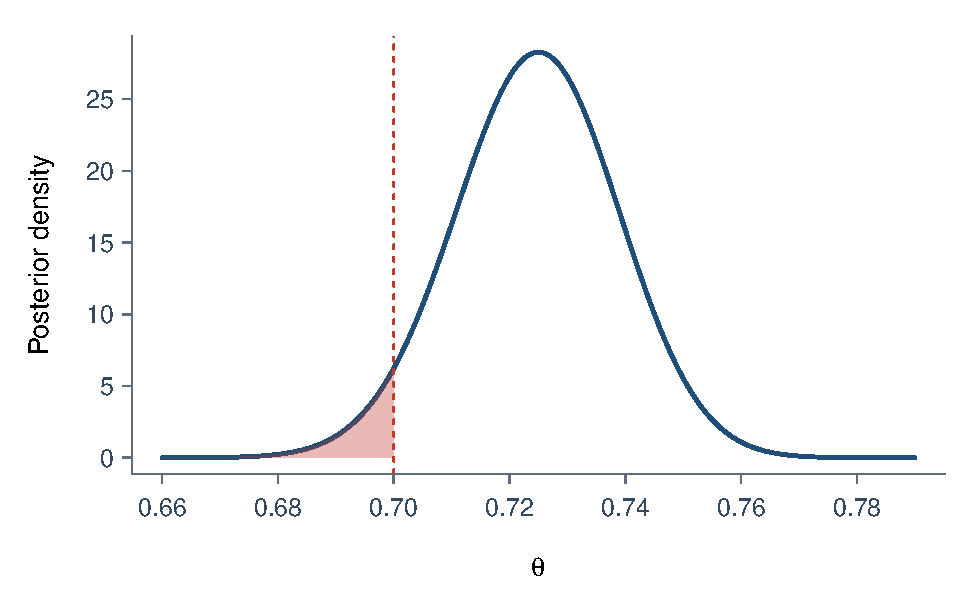
\includegraphics[width=0.7\linewidth]{ex24_posterior.pdf}\end{center}
\emph{For a non-statistician:} ``Given these results, there is about a 96\% chance that the program's graduation rate is above 70\%. Our best estimate is 72.5\%, and it is very likely between 69.7\% and 75.2\%.''

\step{(d) Definitions.}
\begin{itemize}
\item \textbf{p-value} $=\Prob(\text{data at least as extreme as observed}\mid\mathcal H_o\text{ is true})$ --- a probability about the \emph{data}.
\item \textbf{Posterior probability of $\mathcal H_o$} $=\Prob(\mathcal H_o\text{ is true}\mid\text{observed data})$ --- a probability about the \emph{hypothesis}.
\end{itemize}
They condition in opposite directions; a p-value is \emph{not} the probability that $\mathcal H_o$ is true. Here they happen to be close (0.042 vs.\ 0.043), a known coincidence for one-sided tests with flat priors.

\begin{sanity}
The uniform prior gives $\Prob(\mathcal H_o)=0.7$ before seeing data, so the Bayes factor for $\mathcal H_a$ is $\frac{0.957/0.043}{0.3/0.7}\approx52$ --- strong evidence, consistent with the small p-value.
\end{sanity}

\begin{answer}
(a) $z=1.73$, $p\approx0.042$: reject $\mathcal H_o$ at 5\%. \quad (b) Level, one-sided, approximation, independence.\\
(c) $\theta|Y\sim\dist{Beta}(726,276)$; $\Prob(\mathcal H_o|Y)\approx0.043$. \quad (d) $\Prob(\text{data}\mid\mathcal H_o)$ vs.\ $\Prob(\mathcal H_o\mid\text{data})$.
\end{answer}

\begin{takeaway}
``Significant'' does not mean ``large'': the estimated gain is 2.5 points and the interval reaches down to 69.7\%.
\end{takeaway}

% ================================================================= Exercise 25
\exercise{1.25 --- Moderna COVID-19 vaccine efficacy}

\begin{problem}{25}
The initial Moderna COVID-19 vaccine trial [9] produced the data in the table below
\begin{center}
\begin{tabular}{cc|cc}\toprule
\multicolumn{2}{c|}{Placebo} & \multicolumn{2}{c}{Vaccine}\\
Infected & Participants & Infected & Participants\\\midrule
\multicolumn{4}{c}{\emph{(table values and sub-questions missing from our copy of the book --- see note)}}\\\bottomrule
\end{tabular}
\end{center}
\end{problem}

\begin{note}
In our copy of the book the exercise ends at the table header: the numbers and the sub-questions are missing. We use the published primary-analysis data of the trial (Baden et al., \emph{New England Journal of Medicine} 384:403--416, 2021): \textbf{185 of 14{,}073} placebo and \textbf{11 of 14{,}134} vaccine participants had symptomatic COVID-19. The questions below are the natural ones for this chapter; if your copy differs, just change the four numbers in \texttt{ch01.R}.
\end{note}

\begin{restate}
Compare infection rates in the placebo and vaccine groups and estimate vaccine efficacy $\mathrm{VE}=1-\theta_V/\theta_P$: (i) posteriors of both rates, (ii) posterior of VE with a 95\% interval, (iii) probability that VE exceeds 30\% (the FDA's minimum) and 90\%.
\end{restate}

\begin{recall}
\textbf{Monte Carlo}: if we can draw $\theta_P^{(s)}$ and $\theta_V^{(s)}$ from their posteriors, then $g(\theta_P^{(s)},\theta_V^{(s)})$ are draws from the posterior of $g(\theta_P,\theta_V)$, for any function $g$. Averages and percentiles of these draws estimate posterior means and intervals.
\end{recall}

\begin{keyidea}
Two independent beta--binomial models, then simulate VE --- no algebra needed for the ratio.
\end{keyidea}

\solution
\step{(i) Infection rates.}
Uniform priors:
$\theta_P\mid\text{data}\sim\dist{Beta}(1+185,\ 1+14{,}073-185)=\dist{Beta}(186,\,13{,}889)$ and
$\theta_V\mid\text{data}\sim\dist{Beta}(12,\,14{,}124)$; means $\approx1.32\%$ and $0.085\%$.
\step{(ii) Efficacy by simulation.}
\begin{lstlisting}
thP <- rbeta(1e5, 1 + 185, 1 + 14073 - 185)   # placebo infection rate
thV <- rbeta(1e5, 1 + 11,  1 + 14134 - 11)    # vaccine infection rate
VE  <- 1 - thV / thP                          # one VE value per draw
\end{lstlisting}
\begin{center}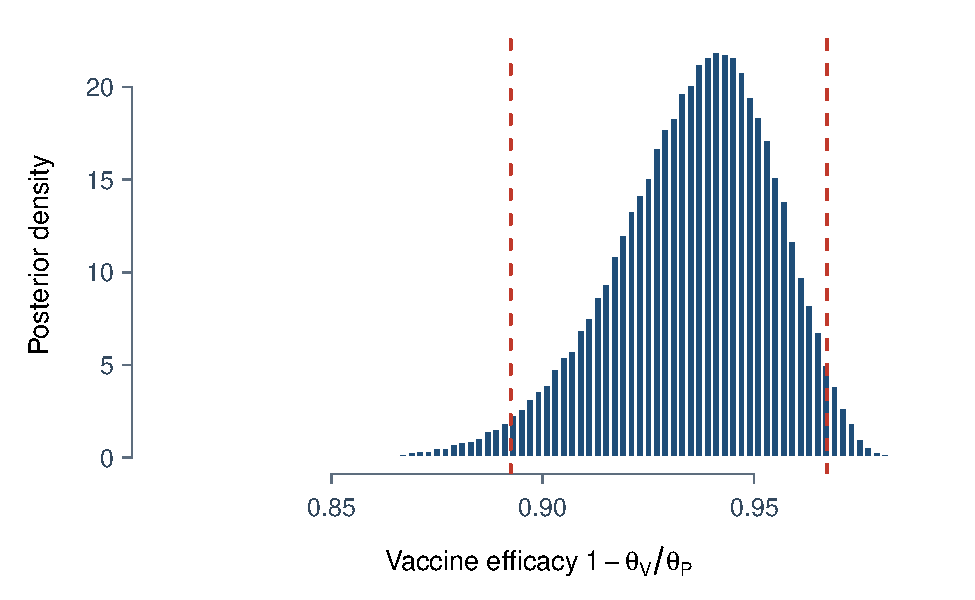
\includegraphics[width=0.72\linewidth]{ex25_efficacy.pdf}\end{center}
Posterior mean $0.935$, median $0.938$, 95\% interval $(0.892,\ 0.967)$.
\step{(iii) Decision-relevant probabilities.}
$\Prob(\mathrm{VE}>0.3\mid\text{data})\approx1$ (no draw out of 100{,}000 fell below), $\Prob(\mathrm{VE}>0.9\mid\text{data})\approx0.95$.

\begin{sanity}
Plug-in check: $1-\frac{11/14134}{185/14073}=1-\frac{0.000778}{0.01315}=0.941$, matching the published estimate of 94.1\% (95\% CI 89.3--96.8\%). \checkmark
\end{sanity}

\begin{answer}
VE posterior mean $\approx93.5\%$, 95\% interval $(89.2\%,\ 96.7\%)$; $\Prob(\mathrm{VE}>30\%)\approx1$, $\Prob(\mathrm{VE}>90\%)\approx0.95$.
\end{answer}

\begin{takeaway}
Monte Carlo makes inference on \emph{any} function of parameters easy (ratios, differences, thresholds) --- the central idea of Chapter 3.
\end{takeaway}

\end{document}
